\documentclass[twoside]{book}

% Packages required by doxygen
\usepackage{calc}
\usepackage{doxygen}
\usepackage{graphicx}
\usepackage[utf8]{inputenc}
\usepackage{makeidx}
\usepackage{multicol}
\usepackage{multirow}
\usepackage{textcomp}
\usepackage[table]{xcolor}

% Font selection
\usepackage[T1]{fontenc}
\usepackage{mathptmx}
\usepackage[scaled=.90]{helvet}
\usepackage{courier}
\usepackage{amssymb}
\usepackage{sectsty}
\renewcommand{\familydefault}{\sfdefault}
\allsectionsfont{%
  \fontseries{bc}\selectfont%
  \color{darkgray}%
}
\renewcommand{\DoxyLabelFont}{%
  \fontseries{bc}\selectfont%
  \color{darkgray}%
}

% Page & text layout
\usepackage{geometry}
\geometry{%
  a4paper,%
  top=2.5cm,%
  bottom=2.5cm,%
  left=2.5cm,%
  right=2.5cm%
}
\tolerance=750
\hfuzz=15pt
\hbadness=750
\setlength{\emergencystretch}{15pt}
\setlength{\parindent}{0cm}
\setlength{\parskip}{0.2cm}
\makeatletter
\renewcommand{\paragraph}{%
  \@startsection{paragraph}{4}{0ex}{-1.0ex}{1.0ex}{%
    \normalfont\normalsize\bfseries\SS@parafont%
  }%
}
\renewcommand{\subparagraph}{%
  \@startsection{subparagraph}{5}{0ex}{-1.0ex}{1.0ex}{%
    \normalfont\normalsize\bfseries\SS@subparafont%
  }%
}
\makeatother

% Headers & footers
\usepackage{fancyhdr}
\pagestyle{fancyplain}
\fancyhead[LE]{\fancyplain{}{\bfseries\thepage}}
\fancyhead[CE]{\fancyplain{}{}}
\fancyhead[RE]{\fancyplain{}{\bfseries\leftmark}}
\fancyhead[LO]{\fancyplain{}{\bfseries\rightmark}}
\fancyhead[CO]{\fancyplain{}{}}
\fancyhead[RO]{\fancyplain{}{\bfseries\thepage}}
\fancyfoot[LE]{\fancyplain{}{}}
\fancyfoot[CE]{\fancyplain{}{}}
\fancyfoot[RE]{\fancyplain{}{\bfseries\scriptsize Generated on Tue Jun 3 2014 15\-:23\-:28 for Project by Doxygen }}
\fancyfoot[LO]{\fancyplain{}{\bfseries\scriptsize Generated on Tue Jun 3 2014 15\-:23\-:28 for Project by Doxygen }}
\fancyfoot[CO]{\fancyplain{}{}}
\fancyfoot[RO]{\fancyplain{}{}}
\renewcommand{\footrulewidth}{0.4pt}
\renewcommand{\chaptermark}[1]{%
  \markboth{#1}{}%
}
\renewcommand{\sectionmark}[1]{%
  \markright{\thesection\ #1}%
}

% Indices & bibliography
\usepackage{natbib}
\usepackage[titles]{tocloft}
\setcounter{tocdepth}{3}
\setcounter{secnumdepth}{5}
\makeindex

% Hyperlinks (required, but should be loaded last)
\usepackage{ifpdf}
\ifpdf
  \usepackage[pdftex,pagebackref=true]{hyperref}
\else
  \usepackage[ps2pdf,pagebackref=true]{hyperref}
\fi
\hypersetup{%
  colorlinks=true,%
  linkcolor=blue,%
  citecolor=blue,%
  unicode%
}

% Custom commands
\newcommand{\clearemptydoublepage}{%
  \newpage{\pagestyle{empty}\cleardoublepage}%
}


%===== C O N T E N T S =====

\begin{document}

% Titlepage & ToC
\hypersetup{pageanchor=false}
\pagenumbering{roman}
\begin{titlepage}
\vspace*{7cm}
\begin{center}%
{\Large Project }\\
\vspace*{1cm}
{\large Generated by Doxygen 1.8.6}\\
\vspace*{0.5cm}
{\small Tue Jun 3 2014 15:23:28}\\
\end{center}
\end{titlepage}
\clearemptydoublepage
\tableofcontents
\clearemptydoublepage
\pagenumbering{arabic}
\hypersetup{pageanchor=true}

%--- Begin generated contents ---
\chapter{Hierarchical Index}
\section{Class Hierarchy}
This inheritance list is sorted roughly, but not completely, alphabetically\-:\begin{DoxyCompactList}
\item \contentsline{section}{Bunka}{\pageref{class_bunka}}{}
\item \contentsline{section}{Farba}{\pageref{struct_farba}}{}
\item \contentsline{section}{Hrac}{\pageref{class_hrac}}{}
\item \contentsline{section}{Kreslic}{\pageref{class_kreslic}}{}
\begin{DoxyCompactList}
\item \contentsline{section}{Kboj}{\pageref{class_kboj}}{}
\item \contentsline{section}{Kinventar}{\pageref{class_kinventar}}{}
\item \contentsline{section}{Kmenu}{\pageref{class_kmenu}}{}
\item \contentsline{section}{Kpole}{\pageref{class_kpole}}{}
\end{DoxyCompactList}
\item \contentsline{section}{Lokacia}{\pageref{class_lokacia}}{}
\item \contentsline{section}{Mechanika}{\pageref{class_mechanika}}{}
\begin{DoxyCompactList}
\item \contentsline{section}{Mboj}{\pageref{class_mboj}}{}
\item \contentsline{section}{Minventar}{\pageref{class_minventar}}{}
\item \contentsline{section}{Mmenu}{\pageref{class_mmenu}}{}
\item \contentsline{section}{Mpole}{\pageref{class_mpole}}{}
\end{DoxyCompactList}
\item \contentsline{section}{Nepriatel}{\pageref{class_nepriatel}}{}
\item \contentsline{section}{Pozicia}{\pageref{struct_pozicia}}{}
\item \contentsline{section}{Predmet}{\pageref{class_predmet}}{}
\begin{DoxyCompactList}
\item \contentsline{section}{Brnenie}{\pageref{class_brnenie}}{}
\item \contentsline{section}{Zbran}{\pageref{class_zbran}}{}
\end{DoxyCompactList}
\item Q\-Main\-Window\begin{DoxyCompactList}
\item \contentsline{section}{Main\-Window}{\pageref{class_main_window}}{}
\end{DoxyCompactList}
\item \contentsline{section}{Ui\-\_\-\-Main\-Window}{\pageref{class_ui___main_window}}{}
\begin{DoxyCompactList}
\item \contentsline{section}{Ui\-:\-:Main\-Window}{\pageref{class_ui_1_1_main_window}}{}
\end{DoxyCompactList}
\end{DoxyCompactList}

\chapter{Class Index}
\section{Class List}
Here are the classes, structs, unions and interfaces with brief descriptions\-:\begin{DoxyCompactList}
\item\contentsline{section}{\hyperlink{class_brnenie}{Brnenie} }{\pageref{class_brnenie}}{}
\item\contentsline{section}{\hyperlink{class_bunka}{Bunka} }{\pageref{class_bunka}}{}
\item\contentsline{section}{\hyperlink{struct_farba}{Farba} \\*Struct ktori sluzi na pracu s farbamy pri vykreslovani }{\pageref{struct_farba}}{}
\item\contentsline{section}{\hyperlink{class_hrac}{Hrac} \\*Trieda ktora definuje vlastnosti hraca }{\pageref{class_hrac}}{}
\item\contentsline{section}{\hyperlink{class_kboj}{Kboj} \\*Tato trieda sa stara o vykreslovanie obrazkovky pri boji }{\pageref{class_kboj}}{}
\item\contentsline{section}{\hyperlink{class_kinventar}{Kinventar} \\*Tato trieda sa stara o vykreslovanie inventara }{\pageref{class_kinventar}}{}
\item\contentsline{section}{\hyperlink{class_kmenu}{Kmenu} \\*Trieda ktora sa stara o vykreslenie menu }{\pageref{class_kmenu}}{}
\item\contentsline{section}{\hyperlink{class_kpole}{Kpole} \\*Trieda ktora sa stara o vykreslovanie herneho pola }{\pageref{class_kpole}}{}
\item\contentsline{section}{\hyperlink{class_kreslic}{Kreslic} \\*Hlavna metoda ktora sa stara o vykreslovanie }{\pageref{class_kreslic}}{}
\item\contentsline{section}{\hyperlink{class_lokacia}{Lokacia} }{\pageref{class_lokacia}}{}
\item\contentsline{section}{\hyperlink{class_ui_1_1_main_window}{Ui\-::\-Main\-Window} }{\pageref{class_ui_1_1_main_window}}{}
\item\contentsline{section}{\hyperlink{class_main_window}{Main\-Window} }{\pageref{class_main_window}}{}
\item\contentsline{section}{\hyperlink{class_mboj}{Mboj} \\*Trieda ktora sa stara o mechaniku boja }{\pageref{class_mboj}}{}
\item\contentsline{section}{\hyperlink{class_mechanika}{Mechanika} \\*Treida ktora sa stara o celu mechaniku hry }{\pageref{class_mechanika}}{}
\item\contentsline{section}{\hyperlink{class_minventar}{Minventar} \\*Trieda ktora sa stara o pracu s inventarom }{\pageref{class_minventar}}{}
\item\contentsline{section}{\hyperlink{class_mmenu}{Mmenu} \\*Trieda ktora sa stara o mechaniku hlavneho menu }{\pageref{class_mmenu}}{}
\item\contentsline{section}{\hyperlink{class_mpole}{Mpole} \\*Trieda ktora sa stara o mechaniku herenho pola }{\pageref{class_mpole}}{}
\item\contentsline{section}{\hyperlink{class_nepriatel}{Nepriatel} \\*Trieda ktora definu nepriatela }{\pageref{class_nepriatel}}{}
\item\contentsline{section}{\hyperlink{struct_pozicia}{Pozicia} \\*Struct definujuci poziciu }{\pageref{struct_pozicia}}{}
\item\contentsline{section}{\hyperlink{class_predmet}{Predmet} }{\pageref{class_predmet}}{}
\item\contentsline{section}{\hyperlink{class_ui___main_window}{Ui\-\_\-\-Main\-Window} }{\pageref{class_ui___main_window}}{}
\item\contentsline{section}{\hyperlink{class_zbran}{Zbran} }{\pageref{class_zbran}}{}
\end{DoxyCompactList}

\chapter{Class Documentation}
\hypertarget{class_brnenie}{\section{Brnenie Class Reference}
\label{class_brnenie}\index{Brnenie@{Brnenie}}
}
Inheritance diagram for Brnenie\-:\begin{figure}[H]
\begin{center}
\leavevmode
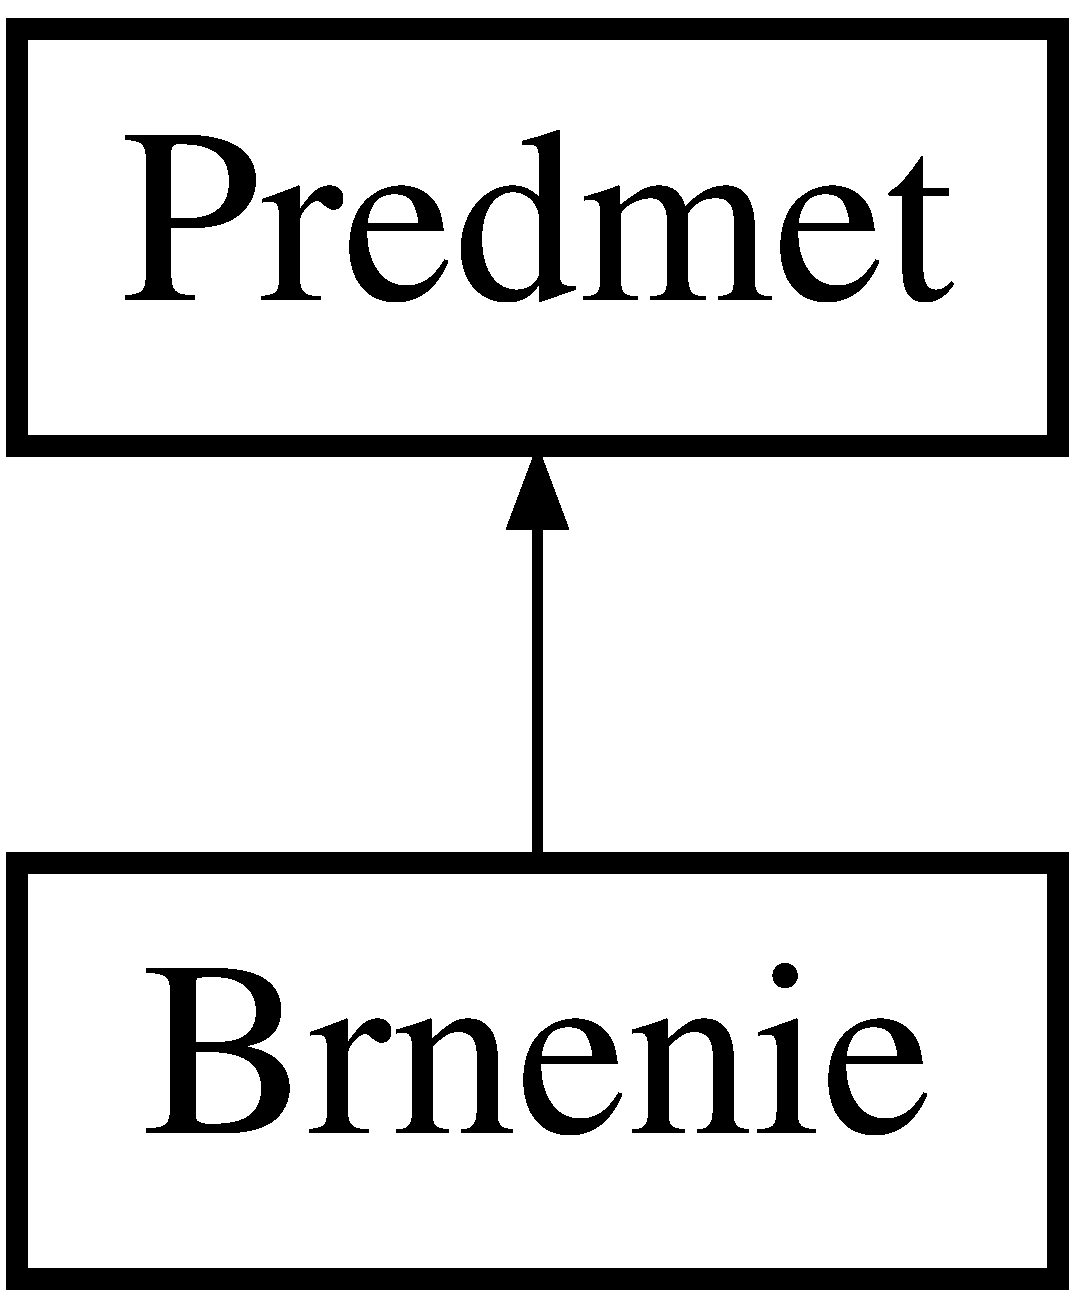
\includegraphics[height=2.000000cm]{class_brnenie}
\end{center}
\end{figure}
\subsection*{Public Member Functions}
\begin{DoxyCompactItemize}
\item 
\hypertarget{class_brnenie_aa87a26f8c7f3c7616a2f2c092ce60514}{{\bfseries Brnenie} (std\-::string nazov, int sila)}\label{class_brnenie_aa87a26f8c7f3c7616a2f2c092ce60514}

\end{DoxyCompactItemize}
\subsection*{Additional Inherited Members}


The documentation for this class was generated from the following files\-:\begin{DoxyCompactItemize}
\item 
Brnenie.\-h\item 
Brnenie.\-cpp\end{DoxyCompactItemize}

\hypertarget{class_bunka}{\section{Bunka Class Reference}
\label{class_bunka}\index{Bunka@{Bunka}}
}
\subsection*{Public Member Functions}
\begin{DoxyCompactItemize}
\item 
\hypertarget{class_bunka_acd2f66e8fd55e45b785381d7868d4e10}{\hyperlink{class_bunka_acd2f66e8fd55e45b785381d7868d4e10}{Bunka} (bool tma)}\label{class_bunka_acd2f66e8fd55e45b785381d7868d4e10}

\begin{DoxyCompactList}\small\item\em hodnota ci tato bunka je prechod do dalsej lokacie \end{DoxyCompactList}\item 
\hypertarget{class_bunka_af30cb993f4512b5dfffb90cf3741cfeb}{void \hyperlink{class_bunka_af30cb993f4512b5dfffb90cf3741cfeb}{Vloz} (\hyperlink{class_brnenie}{Brnenie} $\ast$brn)}\label{class_bunka_af30cb993f4512b5dfffb90cf3741cfeb}

\begin{DoxyCompactList}\small\item\em konstruktor s parametrom ci je bunka odkryta alebo nie \end{DoxyCompactList}\item 
\hypertarget{class_bunka_a5f75753726525606914d3166037eaf59}{void \hyperlink{class_bunka_a5f75753726525606914d3166037eaf59}{Vloz} (\hyperlink{class_zbran}{Zbran} $\ast$zbran)}\label{class_bunka_a5f75753726525606914d3166037eaf59}

\begin{DoxyCompactList}\small\item\em metoda na vlozenie ukazatela na objekt \hyperlink{class_brnenie}{Brnenie} pre atribut m\-\_\-brnenie \end{DoxyCompactList}\item 
\hypertarget{class_bunka_ac6e111643563817eec785e6461516887}{void \hyperlink{class_bunka_ac6e111643563817eec785e6461516887}{Vloz} (bool volno)}\label{class_bunka_ac6e111643563817eec785e6461516887}

\begin{DoxyCompactList}\small\item\em metoda na vlozenie ukazatela na objekt \hyperlink{class_zbran}{Zbran} pre atribut m\-\_\-zbran \end{DoxyCompactList}\item 
\hypertarget{class_bunka_ac21673745a37f9ccee9591348a1a1213}{void \hyperlink{class_bunka_ac21673745a37f9ccee9591348a1a1213}{Vloz} (\hyperlink{class_nepriatel}{Nepriatel} $\ast$nepriatel)}\label{class_bunka_ac21673745a37f9ccee9591348a1a1213}

\begin{DoxyCompactList}\small\item\em metoda na upravenie ci je dana bunka stenaa lebo cesta \end{DoxyCompactList}\item 
\hypertarget{class_bunka_a814b7c399a0a58c46e0a9bfd5a050e30}{void \hyperlink{class_bunka_a814b7c399a0a58c46e0a9bfd5a050e30}{set\-Portal} (bool portal)}\label{class_bunka_a814b7c399a0a58c46e0a9bfd5a050e30}

\begin{DoxyCompactList}\small\item\em metoda na vlozenie ukazatela na objekt \hyperlink{class_nepriatel}{Nepriatel} pre atribut m\-\_\-nepriatel \end{DoxyCompactList}\item 
\hypertarget{class_bunka_ad3d016c5017831e18d22e7266e2f01e9}{bool \hyperlink{class_bunka_ad3d016c5017831e18d22e7266e2f01e9}{get\-Portal} ()}\label{class_bunka_ad3d016c5017831e18d22e7266e2f01e9}

\begin{DoxyCompactList}\small\item\em metoda na nastavenie ci je dana bunka portal, tato hodnota sa uklada do premennej m\-\_\-portal \end{DoxyCompactList}\item 
\hypertarget{class_bunka_a3a206499f4794ae44245b0a13a10694c}{bool \hyperlink{class_bunka_a3a206499f4794ae44245b0a13a10694c}{get\-Tma} ()}\label{class_bunka_a3a206499f4794ae44245b0a13a10694c}

\begin{DoxyCompactList}\small\item\em metoda ktora vracia hodnotu ci je portalom alebo nie, na zaklade premmenej m\-\_\-portal \end{DoxyCompactList}\item 
\hypertarget{class_bunka_a963722f14fa3af3fd246def7092b468c}{void \hyperlink{class_bunka_a963722f14fa3af3fd246def7092b468c}{set\-Tma} (bool tma)}\label{class_bunka_a963722f14fa3af3fd246def7092b468c}

\begin{DoxyCompactList}\small\item\em metoda ktora vrati hodtnotu premmenej m\-\_\-tma \end{DoxyCompactList}\item 
\hypertarget{class_bunka_a741795ec3909545af530c88b3010c51c}{bool \hyperlink{class_bunka_a741795ec3909545af530c88b3010c51c}{get\-Volno} ()}\label{class_bunka_a741795ec3909545af530c88b3010c51c}

\begin{DoxyCompactList}\small\item\em metoda ktora nastavi premennu m\-\_\-tma \end{DoxyCompactList}\item 
\hypertarget{class_bunka_abc925c9c2dd9029f31a64ed54c59377f}{\hyperlink{class_brnenie}{Brnenie} $\ast$ \hyperlink{class_bunka_abc925c9c2dd9029f31a64ed54c59377f}{get\-Brnenie} ()}\label{class_bunka_abc925c9c2dd9029f31a64ed54c59377f}

\begin{DoxyCompactList}\small\item\em metoda ktora vrati obsah hodnoty m\-\_\-volno \end{DoxyCompactList}\item 
\hypertarget{class_bunka_a6b241bae5b391e76ba00ed250dd61d2c}{\hyperlink{class_zbran}{Zbran} $\ast$ \hyperlink{class_bunka_a6b241bae5b391e76ba00ed250dd61d2c}{get\-Zbran} ()}\label{class_bunka_a6b241bae5b391e76ba00ed250dd61d2c}

\begin{DoxyCompactList}\small\item\em metoda ktora vrati obsah premmenej m\-\_\-brnenie \end{DoxyCompactList}\item 
\hypertarget{class_bunka_a81cf6cc8e4809fcdfa2b3b3bfeea4d79}{\hyperlink{class_nepriatel}{Nepriatel} $\ast$ \hyperlink{class_bunka_a81cf6cc8e4809fcdfa2b3b3bfeea4d79}{get\-Nepriatel} ()}\label{class_bunka_a81cf6cc8e4809fcdfa2b3b3bfeea4d79}

\begin{DoxyCompactList}\small\item\em metoda ktora vrati obsah premennej m\-\_\-zbran \end{DoxyCompactList}\end{DoxyCompactItemize}


The documentation for this class was generated from the following files\-:\begin{DoxyCompactItemize}
\item 
Bunka.\-h\item 
Bunka.\-cpp\end{DoxyCompactItemize}

\hypertarget{struct_farba}{\section{Farba Struct Reference}
\label{struct_farba}\index{Farba@{Farba}}
}


struct ktori sluzi na pracu s farbamy pri vykreslovani  




{\ttfamily \#include $<$Farba.\-h$>$}

\subsection*{Public Member Functions}
\begin{DoxyCompactItemize}
\item 
\hypertarget{struct_farba_a5f58214fe6a6962b92e96c667d8c5cbd}{{\bfseries Farba} (const G\-Lbyte r, const G\-Lbyte g, const G\-Lbyte b)}\label{struct_farba_a5f58214fe6a6962b92e96c667d8c5cbd}

\end{DoxyCompactItemize}
\subsection*{Public Attributes}
\begin{DoxyCompactItemize}
\item 
\hypertarget{struct_farba_a8d6af6c200e171f6e77ffd26a870a93e}{G\-Lbyte {\bfseries r}}\label{struct_farba_a8d6af6c200e171f6e77ffd26a870a93e}

\item 
\hypertarget{struct_farba_abb0eaf65fe825f8bc6d8dd4df3757352}{G\-Lbyte {\bfseries g}}\label{struct_farba_abb0eaf65fe825f8bc6d8dd4df3757352}

\item 
\hypertarget{struct_farba_adbd8d5299c2071e336db215ab1dd35d8}{G\-Lbyte {\bfseries b}}\label{struct_farba_adbd8d5299c2071e336db215ab1dd35d8}

\end{DoxyCompactItemize}


\subsection{Detailed Description}
struct ktori sluzi na pracu s farbamy pri vykreslovani 

The documentation for this struct was generated from the following file\-:\begin{DoxyCompactItemize}
\item 
Farba.\-h\end{DoxyCompactItemize}

\hypertarget{class_hrac}{\section{Hrac Class Reference}
\label{class_hrac}\index{Hrac@{Hrac}}
}


trieda ktora definuje vlastnosti hraca  




{\ttfamily \#include $<$hrac.\-h$>$}

\subsection*{Public Member Functions}
\begin{DoxyCompactItemize}
\item 
\hypertarget{class_hrac_a47fe983c204445b3f1c638c5ef799df4}{\hyperlink{class_hrac_a47fe983c204445b3f1c638c5ef799df4}{Hrac} ()}\label{class_hrac_a47fe983c204445b3f1c638c5ef799df4}

\begin{DoxyCompactList}\small\item\em premenna typu ukazatel na objekt \hyperlink{class_zbran}{Zbran}, ktoru hrac prave teraz pouziva \end{DoxyCompactList}\item 
\hypertarget{class_hrac_a6ea5accaf15f5712076c8dcc6c1b09d1}{\hyperlink{struct_pozicia}{Pozicia} \hyperlink{class_hrac_a6ea5accaf15f5712076c8dcc6c1b09d1}{get\-Pozicia} ()}\label{class_hrac_a6ea5accaf15f5712076c8dcc6c1b09d1}

\begin{DoxyCompactList}\small\item\em bezparametricky konstruktor, iny nieje potrebny \end{DoxyCompactList}\item 
\hypertarget{class_hrac_a6c9c09d4dafa26517536e914f7d57fd6}{void \hyperlink{class_hrac_a6c9c09d4dafa26517536e914f7d57fd6}{set\-Pozicia} (\hyperlink{struct_pozicia}{Pozicia} poz)}\label{class_hrac_a6c9c09d4dafa26517536e914f7d57fd6}

\begin{DoxyCompactList}\small\item\em metoda ktora vracia poziciu an ktorej sa hrac nachadza \end{DoxyCompactList}\item 
\hypertarget{class_hrac_afc0949f3d26024f6315f5bb054c1346f}{\hyperlink{class_zbran}{Zbran} $\ast$ \hyperlink{class_hrac_afc0949f3d26024f6315f5bb054c1346f}{get\-Zbran} ()}\label{class_hrac_afc0949f3d26024f6315f5bb054c1346f}

\begin{DoxyCompactList}\small\item\em metoda ktora nastavuje premennu m\-\_\-pozicia \end{DoxyCompactList}\item 
\hypertarget{class_hrac_a69d7cd6bc722e35604d3c8d60be001f7}{\hyperlink{class_brnenie}{Brnenie} $\ast$ \hyperlink{class_hrac_a69d7cd6bc722e35604d3c8d60be001f7}{get\-Brnenie} ()}\label{class_hrac_a69d7cd6bc722e35604d3c8d60be001f7}

\begin{DoxyCompactList}\small\item\em metoda ktora vracia ukazatel na objekt \hyperlink{class_zbran}{Zbran} ktory hrac pouziva \end{DoxyCompactList}\item 
\hypertarget{class_hrac_a08592e19c7078a31e2f8edbd55ffb58f}{int \hyperlink{class_hrac_a08592e19c7078a31e2f8edbd55ffb58f}{get\-Zivot} ()}\label{class_hrac_a08592e19c7078a31e2f8edbd55ffb58f}

\begin{DoxyCompactList}\small\item\em meotda ktora vracia ukazatel na objekt \hyperlink{class_brnenie}{Brnenie} ktory hrac pouziva \end{DoxyCompactList}\item 
\hypertarget{class_hrac_ad36a26d588dc0c95435ab20304e62dda}{void \hyperlink{class_hrac_ad36a26d588dc0c95435ab20304e62dda}{pridaj} (\hyperlink{class_zbran}{Zbran} $\ast$zbran)}\label{class_hrac_ad36a26d588dc0c95435ab20304e62dda}

\begin{DoxyCompactList}\small\item\em metoda ktora vracia premennu m\-\_\-zivot \end{DoxyCompactList}\item 
\hypertarget{class_hrac_a349a8dd0bc3c75df4f3389f7c2fb8021}{void \hyperlink{class_hrac_a349a8dd0bc3c75df4f3389f7c2fb8021}{pridaj} (\hyperlink{class_brnenie}{Brnenie} $\ast$brn)}\label{class_hrac_a349a8dd0bc3c75df4f3389f7c2fb8021}

\begin{DoxyCompactList}\small\item\em metoda ktora prida no vektora m\-\_\-inventar objekt predany v parametre, a pokial je lepsi ako objekt v premennej m\-\_\-zbran tak ho nahradi \end{DoxyCompactList}\item 
\hypertarget{class_hrac_a191eb129196e1ffc5b191da6a0d78950}{std\-::vector$<$ \hyperlink{class_predmet}{Predmet} $\ast$ $>$ \hyperlink{class_hrac_a191eb129196e1ffc5b191da6a0d78950}{get\-Inventar} ()}\label{class_hrac_a191eb129196e1ffc5b191da6a0d78950}

\begin{DoxyCompactList}\small\item\em metoda ktora prida no vektora m\-\_\-inventar objekt predany v parametre, a pokial je lepsi ako objekt v premennej m\-\_\-brnenie tak ho nahradi \end{DoxyCompactList}\end{DoxyCompactItemize}


\subsection{Detailed Description}
trieda ktora definuje vlastnosti hraca 

The documentation for this class was generated from the following files\-:\begin{DoxyCompactItemize}
\item 
hrac.\-h\item 
hrac.\-cpp\end{DoxyCompactItemize}

\hypertarget{class_kboj}{\section{Kboj Class Reference}
\label{class_kboj}\index{Kboj@{Kboj}}
}


tato trieda sa stara o vykreslovanie obrazkovky pri boji  




{\ttfamily \#include $<$kboj.\-h$>$}

Inheritance diagram for Kboj\-:\begin{figure}[H]
\begin{center}
\leavevmode
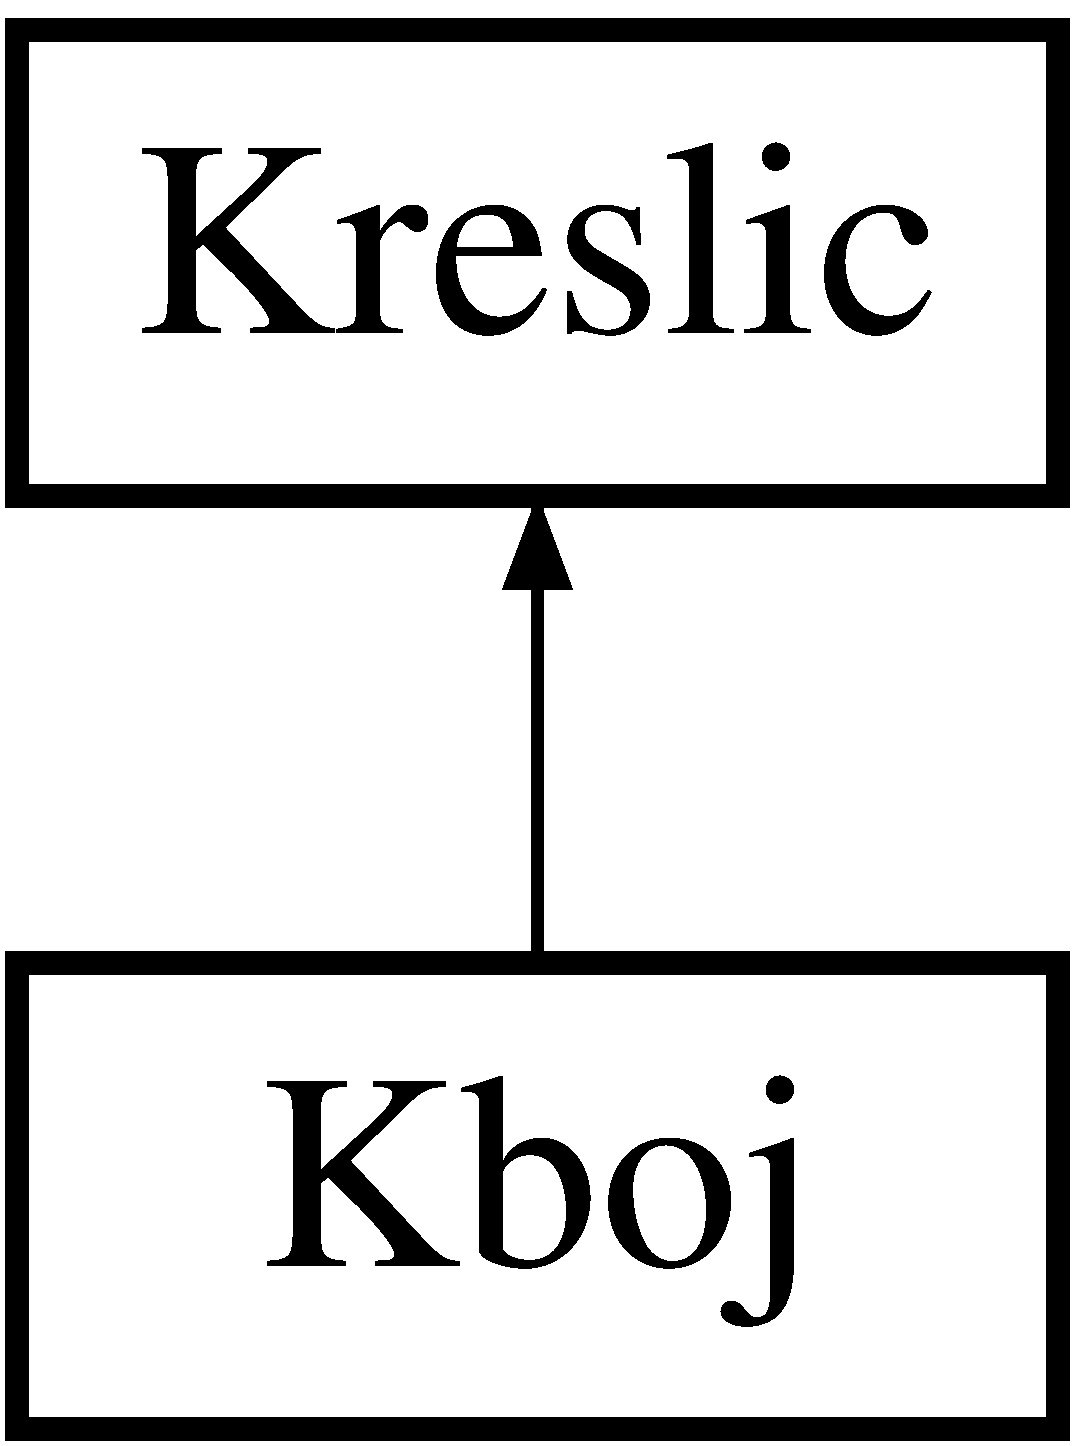
\includegraphics[height=2.000000cm]{class_kboj}
\end{center}
\end{figure}
\subsection*{Public Member Functions}
\begin{DoxyCompactItemize}
\item 
\hypertarget{class_kboj_a7d88c71591763faf1cc9c33dc4aa84b5}{\hyperlink{class_kboj_a7d88c71591763faf1cc9c33dc4aa84b5}{Kboj} (\hyperlink{class_lokacia}{Lokacia} $\ast$lok, \hyperlink{class_hrac}{Hrac} $\ast$hrac)}\label{class_kboj_a7d88c71591763faf1cc9c33dc4aa84b5}

\begin{DoxyCompactList}\small\item\em ukazatel na hraca \end{DoxyCompactList}\item 
\hypertarget{class_kboj_af62fd0316418ce641fe7e388df88fdfd}{void \hyperlink{class_kboj_af62fd0316418ce641fe7e388df88fdfd}{Kresli} ()}\label{class_kboj_af62fd0316418ce641fe7e388df88fdfd}

\begin{DoxyCompactList}\small\item\em parametricky konstruktor ktori ulozi udaje z paramtrov do atributov \end{DoxyCompactList}\item 
\hypertarget{class_kboj_aca5a9f94fa87d6ccf1cd3f0ad0e0cfdb}{\hyperlink{class_nepriatel}{Nepriatel} $\ast$ \hyperlink{class_kboj_aca5a9f94fa87d6ccf1cd3f0ad0e0cfdb}{najdi} ()}\label{class_kboj_aca5a9f94fa87d6ccf1cd3f0ad0e0cfdb}

\begin{DoxyCompactList}\small\item\em metoda ktora sa stara o samtoen vykreslovanie \end{DoxyCompactList}\end{DoxyCompactItemize}
\subsection*{Additional Inherited Members}


\subsection{Detailed Description}
tato trieda sa stara o vykreslovanie obrazkovky pri boji 

The documentation for this class was generated from the following files\-:\begin{DoxyCompactItemize}
\item 
kboj.\-h\item 
kboj.\-cpp\end{DoxyCompactItemize}

\hypertarget{class_kinventar}{\section{Kinventar Class Reference}
\label{class_kinventar}\index{Kinventar@{Kinventar}}
}


tato trieda sa stara o vykreslovanie inventara  




{\ttfamily \#include $<$Kinventar.\-h$>$}

Inheritance diagram for Kinventar\-:\begin{figure}[H]
\begin{center}
\leavevmode
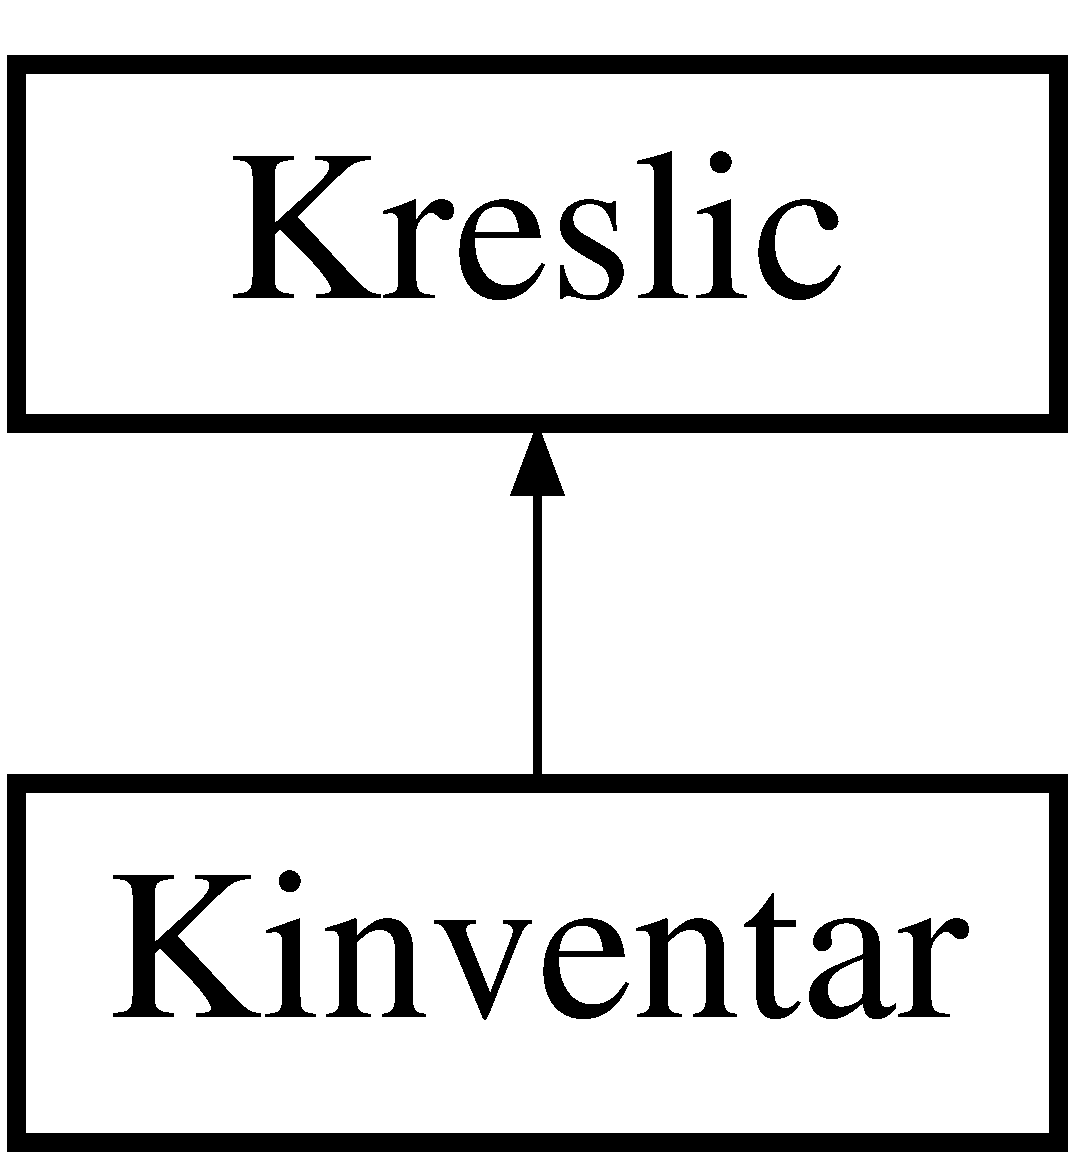
\includegraphics[height=2.000000cm]{class_kinventar}
\end{center}
\end{figure}
\subsection*{Public Member Functions}
\begin{DoxyCompactItemize}
\item 
\hypertarget{class_kinventar_ab811ba9d0843cdd16fd45bf5461f1d8c}{\hyperlink{class_kinventar_ab811ba9d0843cdd16fd45bf5461f1d8c}{Kinventar} (\hyperlink{class_hrac}{Hrac} $\ast$hrac)}\label{class_kinventar_ab811ba9d0843cdd16fd45bf5461f1d8c}

\begin{DoxyCompactList}\small\item\em tato premenna obsahuje ukazatel an hraca ktoreho inventar sa ma vykreslit \end{DoxyCompactList}\item 
\hypertarget{class_kinventar_a4177cf7447c74ff5d582c415146845e4}{void \hyperlink{class_kinventar_a4177cf7447c74ff5d582c415146845e4}{Kresli} ()}\label{class_kinventar_a4177cf7447c74ff5d582c415146845e4}

\begin{DoxyCompactList}\small\item\em parametricky konstruktor ktori ulozit ukazatel na hraca \end{DoxyCompactList}\end{DoxyCompactItemize}
\subsection*{Additional Inherited Members}


\subsection{Detailed Description}
tato trieda sa stara o vykreslovanie inventara 

The documentation for this class was generated from the following files\-:\begin{DoxyCompactItemize}
\item 
Kinventar.\-h\item 
Kinventar.\-cpp\end{DoxyCompactItemize}

\hypertarget{class_kmenu}{\section{Kmenu Class Reference}
\label{class_kmenu}\index{Kmenu@{Kmenu}}
}


trieda ktora sa stara o vykreslenie menu  




{\ttfamily \#include $<$Kmenu.\-h$>$}

Inheritance diagram for Kmenu\-:\begin{figure}[H]
\begin{center}
\leavevmode
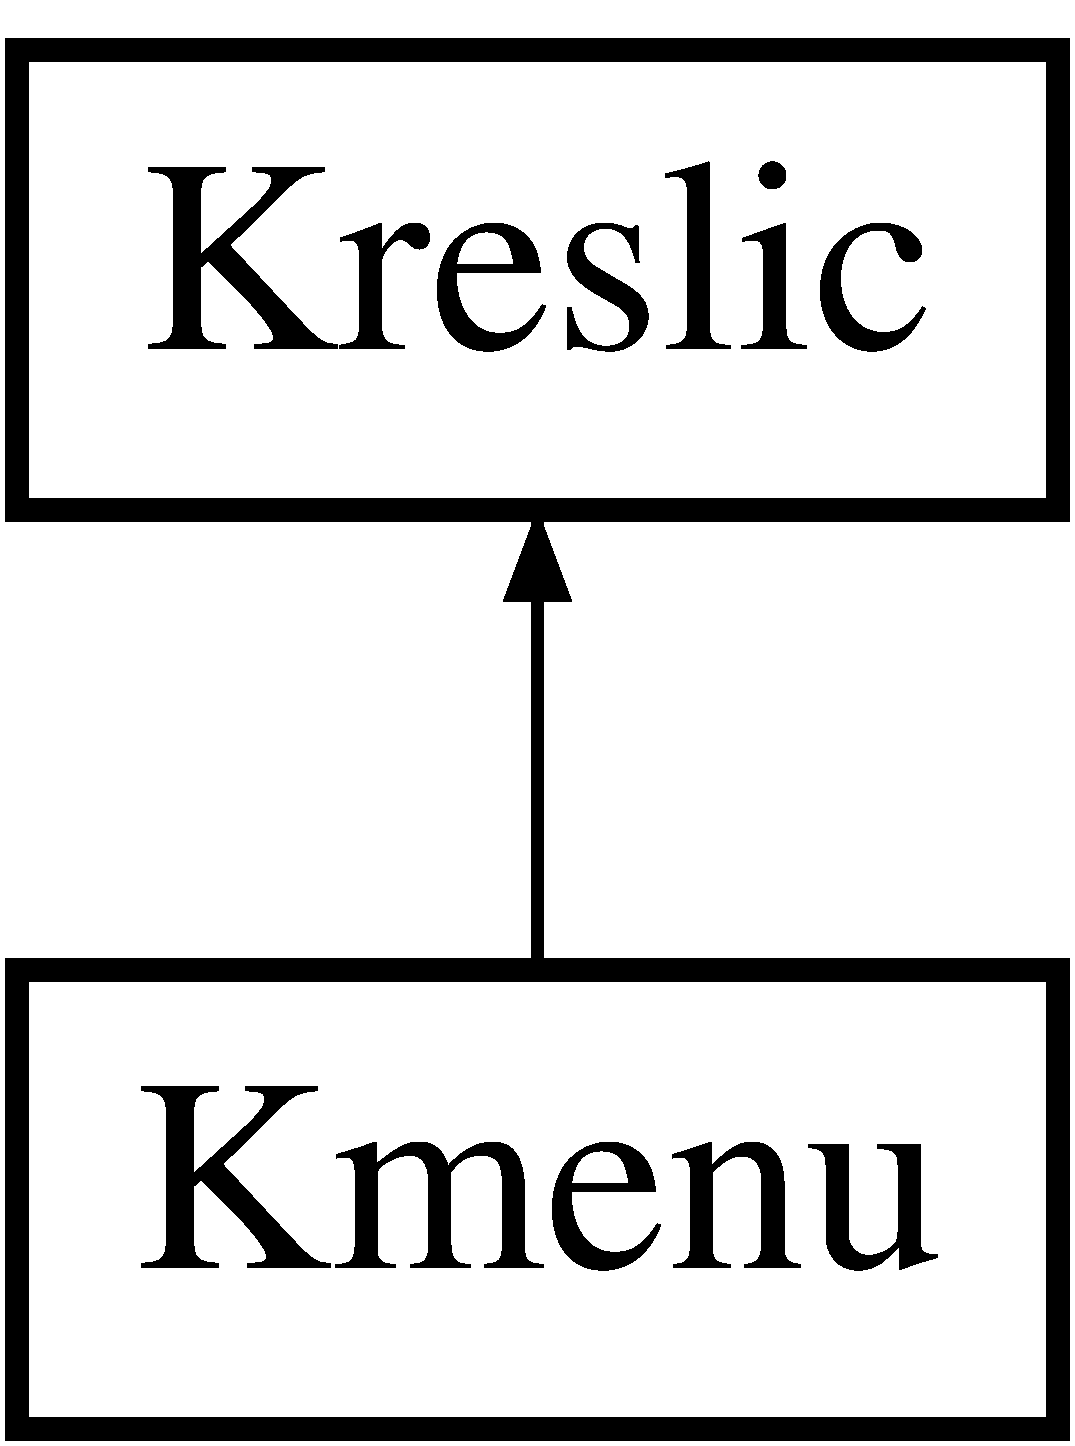
\includegraphics[height=2.000000cm]{class_kmenu}
\end{center}
\end{figure}
\subsection*{Public Member Functions}
\begin{DoxyCompactItemize}
\item 
\hypertarget{class_kmenu_ad8d318b904d5b90a0a01645527b0e8ba}{void \hyperlink{class_kmenu_ad8d318b904d5b90a0a01645527b0e8ba}{Kresli} ()}\label{class_kmenu_ad8d318b904d5b90a0a01645527b0e8ba}

\begin{DoxyCompactList}\small\item\em bezparametricky konstruktor \end{DoxyCompactList}\end{DoxyCompactItemize}
\subsection*{Additional Inherited Members}


\subsection{Detailed Description}
trieda ktora sa stara o vykreslenie menu 

The documentation for this class was generated from the following files\-:\begin{DoxyCompactItemize}
\item 
Kmenu.\-h\item 
Kmenu.\-cpp\end{DoxyCompactItemize}

\hypertarget{class_kpole}{\section{Kpole Class Reference}
\label{class_kpole}\index{Kpole@{Kpole}}
}


trieda ktora sa stara o vykreslovanie herneho pola  




{\ttfamily \#include $<$Kpole.\-h$>$}

Inheritance diagram for Kpole\-:\begin{figure}[H]
\begin{center}
\leavevmode
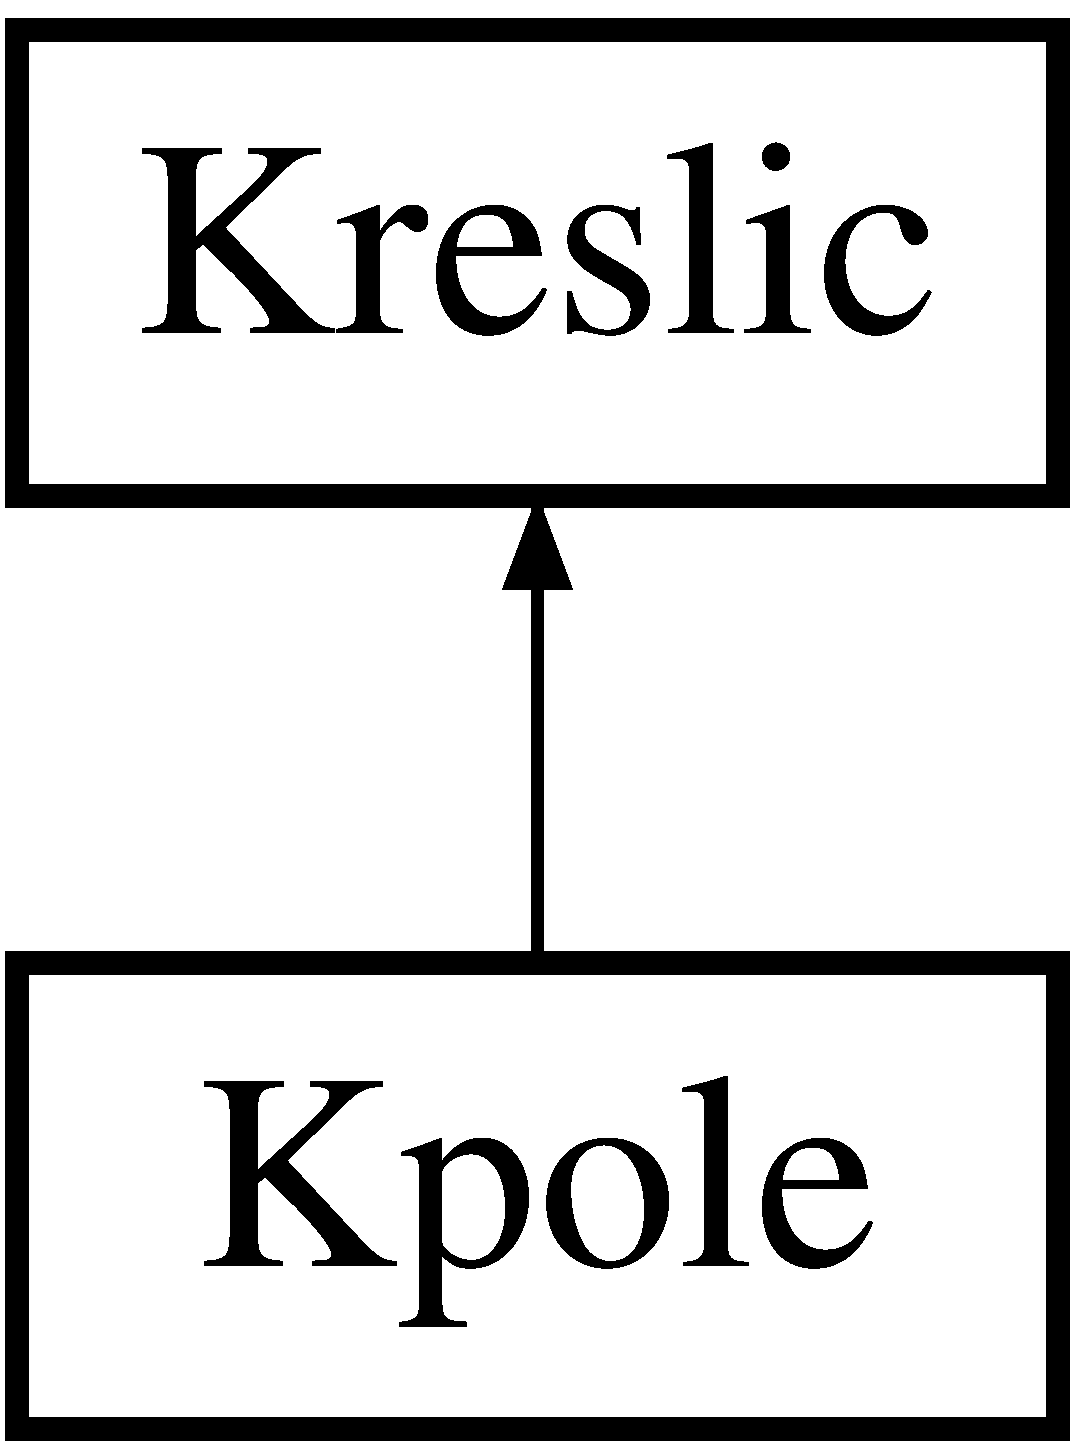
\includegraphics[height=2.000000cm]{class_kpole}
\end{center}
\end{figure}
\subsection*{Public Member Functions}
\begin{DoxyCompactItemize}
\item 
\hypertarget{class_kpole_a63d5f5dc29507cbe8ce0a199ff4f5e8f}{\hyperlink{class_kpole_a63d5f5dc29507cbe8ce0a199ff4f5e8f}{Kpole} (\hyperlink{class_lokacia}{Lokacia} $\ast$lokacia, \hyperlink{class_hrac}{Hrac} $\ast$hrac)}\label{class_kpole_a63d5f5dc29507cbe8ce0a199ff4f5e8f}

\begin{DoxyCompactList}\small\item\em premenna osbahujuca ukazatel an hraca \end{DoxyCompactList}\item 
\hypertarget{class_kpole_a8cc0da29e42f4f637f9be412e58f3f7f}{void \hyperlink{class_kpole_a8cc0da29e42f4f637f9be412e58f3f7f}{Kresli} ()}\label{class_kpole_a8cc0da29e42f4f637f9be412e58f3f7f}

\begin{DoxyCompactList}\small\item\em parametricky konstruktor ktori parametre ulozi do atributov \end{DoxyCompactList}\item 
\hypertarget{class_kpole_a5656de037f98ce24e0d1b2e48255a996}{void \hyperlink{class_kpole_a5656de037f98ce24e0d1b2e48255a996}{Hraca} (\hyperlink{struct_pozicia}{Pozicia} poz)}\label{class_kpole_a5656de037f98ce24e0d1b2e48255a996}

\begin{DoxyCompactList}\small\item\em metoda ktora sa stara o vykreslovanie \end{DoxyCompactList}\item 
\hypertarget{class_kpole_a3b00d8874bed3d779bb07a42a0c26a79}{void \hyperlink{class_kpole_a3b00d8874bed3d779bb07a42a0c26a79}{Nepriatela} (\hyperlink{struct_pozicia}{Pozicia} poz)}\label{class_kpole_a3b00d8874bed3d779bb07a42a0c26a79}

\begin{DoxyCompactList}\small\item\em pomocna metoda ktora vykresli harac na pozicii zadanej v parametre \end{DoxyCompactList}\item 
\hypertarget{class_kpole_a412c877b0caf432f0e9b4a53b3b9e5e7}{void \hyperlink{class_kpole_a412c877b0caf432f0e9b4a53b3b9e5e7}{Cesta} (\hyperlink{struct_pozicia}{Pozicia} prva, \hyperlink{struct_pozicia}{Pozicia} druha)}\label{class_kpole_a412c877b0caf432f0e9b4a53b3b9e5e7}

\begin{DoxyCompactList}\small\item\em pomocna metoda ktora vykresli nepriatela na zadanej pozicii \end{DoxyCompactList}\item 
\hypertarget{class_kpole_a452b8134669f24dfe94ab933d5633fdb}{void \hyperlink{class_kpole_a452b8134669f24dfe94ab933d5633fdb}{Nic} (\hyperlink{struct_pozicia}{Pozicia} prva, \hyperlink{struct_pozicia}{Pozicia} druha)}\label{class_kpole_a452b8134669f24dfe94ab933d5633fdb}

\begin{DoxyCompactList}\small\item\em pomocna metoda ktora vykresli cestu na zadanej pozicii \end{DoxyCompactList}\item 
\hypertarget{class_kpole_ab513ed3e38adfc27226dcb364d11dbdc}{void \hyperlink{class_kpole_ab513ed3e38adfc27226dcb364d11dbdc}{Stena} (\hyperlink{struct_pozicia}{Pozicia} prva, \hyperlink{struct_pozicia}{Pozicia} druha)}\label{class_kpole_ab513ed3e38adfc27226dcb364d11dbdc}

\begin{DoxyCompactList}\small\item\em pomozna metoda ktora vykresli tmu \end{DoxyCompactList}\item 
\hypertarget{class_kpole_a2982cdfc9f891b35a1651ce62b2eec02}{void \hyperlink{class_kpole_a2982cdfc9f891b35a1651ce62b2eec02}{Brnenie} (\hyperlink{struct_pozicia}{Pozicia} poz)}\label{class_kpole_a2982cdfc9f891b35a1651ce62b2eec02}

\begin{DoxyCompactList}\small\item\em pomocna metoda ktora vykresli stenu \end{DoxyCompactList}\item 
\hypertarget{class_kpole_ab4987bb1f9bfe8e9721a18054a128bf6}{void \hyperlink{class_kpole_ab4987bb1f9bfe8e9721a18054a128bf6}{Zbran} (\hyperlink{struct_pozicia}{Pozicia} poz)}\label{class_kpole_ab4987bb1f9bfe8e9721a18054a128bf6}

\begin{DoxyCompactList}\small\item\em pomocna metoda ktora vykresli brnenie \end{DoxyCompactList}\item 
\hypertarget{class_kpole_aa668c2502a5a4ecdadeb7d7cbaf2fe1e}{void \hyperlink{class_kpole_aa668c2502a5a4ecdadeb7d7cbaf2fe1e}{portal} (\hyperlink{struct_pozicia}{Pozicia} poz)}\label{class_kpole_aa668c2502a5a4ecdadeb7d7cbaf2fe1e}

\begin{DoxyCompactList}\small\item\em pomocna metoda ktora vykresli zbran \end{DoxyCompactList}\end{DoxyCompactItemize}
\subsection*{Additional Inherited Members}


\subsection{Detailed Description}
trieda ktora sa stara o vykreslovanie herneho pola 

The documentation for this class was generated from the following files\-:\begin{DoxyCompactItemize}
\item 
Kpole.\-h\item 
Kpole.\-cpp\end{DoxyCompactItemize}

\hypertarget{class_kreslic}{\section{Kreslic Class Reference}
\label{class_kreslic}\index{Kreslic@{Kreslic}}
}


hlavna metoda ktora sa stara o vykreslovanie  




{\ttfamily \#include $<$Kreslic.\-h$>$}

Inheritance diagram for Kreslic\-:\begin{figure}[H]
\begin{center}
\leavevmode
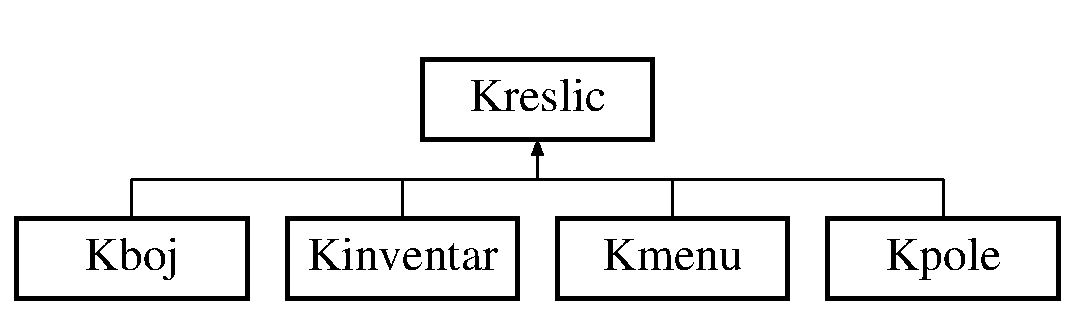
\includegraphics[height=2.000000cm]{class_kreslic}
\end{center}
\end{figure}
\subsection*{Public Member Functions}
\begin{DoxyCompactItemize}
\item 
\hypertarget{class_kreslic_ab0f01f44293ef4d5cb0d3b15017cbcd0}{\hyperlink{class_kreslic_ab0f01f44293ef4d5cb0d3b15017cbcd0}{Kreslic} ()}\label{class_kreslic_ab0f01f44293ef4d5cb0d3b15017cbcd0}

\begin{DoxyCompactList}\small\item\em metoda ktora sa stara o vykreslenie textu \end{DoxyCompactList}\item 
\hypertarget{class_kreslic_a11e344af477f3bf2724ff871c6291768}{void \hyperlink{class_kreslic_a11e344af477f3bf2724ff871c6291768}{resize} (int w, int h)}\label{class_kreslic_a11e344af477f3bf2724ff871c6291768}

\begin{DoxyCompactList}\small\item\em bezparametrcky konstruktor \end{DoxyCompactList}\item 
\hypertarget{class_kreslic_ae719429a9a3a3e2a95f7b606ac79d307}{void \hyperlink{class_kreslic_ae719429a9a3a3e2a95f7b606ac79d307}{display} ()}\label{class_kreslic_ae719429a9a3a3e2a95f7b606ac79d307}

\begin{DoxyCompactList}\small\item\em metoda ktora riesi zmenu velkosti ukna \end{DoxyCompactList}\item 
\hypertarget{class_kreslic_a4259d894b56e1c264f3eb5b1db9352f7}{virtual void \hyperlink{class_kreslic_a4259d894b56e1c264f3eb5b1db9352f7}{Kresli} ()=0}\label{class_kreslic_a4259d894b56e1c264f3eb5b1db9352f7}

\begin{DoxyCompactList}\small\item\em metoda ktora sa stara o vykreslenie toho co sa prave zapisalo an vykreslenie \end{DoxyCompactList}\item 
\hypertarget{class_kreslic_aa4c9c244b81ca405fccb2b5d0fa845cd}{void \hyperlink{class_kreslic_aa4c9c244b81ca405fccb2b5d0fa845cd}{pis} (std\-::string)}\label{class_kreslic_aa4c9c244b81ca405fccb2b5d0fa845cd}

\begin{DoxyCompactList}\small\item\em abstraktna metoda ktora sluzi na vykreslenie toho daneho prostredia \end{DoxyCompactList}\end{DoxyCompactItemize}
\subsection*{Protected Member Functions}
\begin{DoxyCompactItemize}
\item 
\hypertarget{class_kreslic_a09d5dd2518b9ccf301d0c92e15ec02f5}{void \hyperlink{class_kreslic_a09d5dd2518b9ccf301d0c92e15ec02f5}{Kruh} ()}\label{class_kreslic_a09d5dd2518b9ccf301d0c92e15ec02f5}

\begin{DoxyCompactList}\small\item\em vektor strungov ktore obsahuju polozky pre vykreslenie legendy \end{DoxyCompactList}\item 
\hypertarget{class_kreslic_a44f827cd0eda38a2067cab7657fd537e}{void \hyperlink{class_kreslic_a44f827cd0eda38a2067cab7657fd537e}{Stvorec} (\hyperlink{struct_pozicia}{Pozicia} prva, \hyperlink{struct_pozicia}{Pozicia} druha, \hyperlink{struct_farba}{Farba} farb)}\label{class_kreslic_a44f827cd0eda38a2067cab7657fd537e}

\begin{DoxyCompactList}\small\item\em metoda ktora sa stara o vykreslenie kruhu \end{DoxyCompactList}\item 
\hypertarget{class_kreslic_afba0442f11b078d7272fb81047480fbf}{void \hyperlink{class_kreslic_afba0442f11b078d7272fb81047480fbf}{Text} (std\-::string text, \hyperlink{struct_pozicia}{Pozicia} poz, \hyperlink{struct_farba}{Farba} farb)}\label{class_kreslic_afba0442f11b078d7272fb81047480fbf}

\begin{DoxyCompactList}\small\item\em metoda ktora sa stara o vykreslenie stvorca \end{DoxyCompactList}\end{DoxyCompactItemize}
\subsection*{Protected Attributes}
\begin{DoxyCompactItemize}
\item 
\hypertarget{class_kreslic_a1fb614c273d51f93c86f8589d5d91f1d}{int {\bfseries m\-\_\-velkost}}\label{class_kreslic_a1fb614c273d51f93c86f8589d5d91f1d}

\item 
\hypertarget{class_kreslic_a8773018fd134429d99f9d999bda4c424}{int {\bfseries pom}}\label{class_kreslic_a8773018fd134429d99f9d999bda4c424}

\item 
\hypertarget{class_kreslic_a10efd37dd45c5ad887835eae6e3c463a}{\hyperlink{class_lokacia}{Lokacia} $\ast$ \hyperlink{class_kreslic_a10efd37dd45c5ad887835eae6e3c463a}{m\-\_\-lokacia}}\label{class_kreslic_a10efd37dd45c5ad887835eae6e3c463a}

\begin{DoxyCompactList}\small\item\em premenna ktora sa zadefinuje v konstruktore ktora urcuje velkost vsetko co sa vykresluje a pomocna premenna pom ktora sa pouziva vsade \end{DoxyCompactList}\item 
\hypertarget{class_kreslic_ab36883117907f55e5c3af6e13dda3d6e}{\hyperlink{class_lokacia}{Lokacia} $\ast$ \hyperlink{class_kreslic_ab36883117907f55e5c3af6e13dda3d6e}{m\-\_\-mapa}}\label{class_kreslic_ab36883117907f55e5c3af6e13dda3d6e}

\begin{DoxyCompactList}\small\item\em premenna typu ukazatel an objekt triedy \hyperlink{class_lokacia}{Lokacia} ktora sa prave pouziva \end{DoxyCompactList}\item 
\hypertarget{class_kreslic_ade0686fa0ef71327df9ff89c3e50f015}{std\-::vector$<$ std\-::string $>$ \hyperlink{class_kreslic_ade0686fa0ef71327df9ff89c3e50f015}{m\-\_\-polozky}}\label{class_kreslic_ade0686fa0ef71327df9ff89c3e50f015}

\begin{DoxyCompactList}\small\item\em premenna typu ukazatel an objekt triedy \hyperlink{class_lokacia}{Lokacia} ktora sa prave pouziva \end{DoxyCompactList}\end{DoxyCompactItemize}


\subsection{Detailed Description}
hlavna metoda ktora sa stara o vykreslovanie 

The documentation for this class was generated from the following files\-:\begin{DoxyCompactItemize}
\item 
Kreslic.\-h\item 
Kreslic.\-cpp\end{DoxyCompactItemize}

\hypertarget{class_lokacia}{\section{Lokacia Class Reference}
\label{class_lokacia}\index{Lokacia@{Lokacia}}
}
\subsection*{Public Member Functions}
\begin{DoxyCompactItemize}
\item 
\hypertarget{class_lokacia_a771d3fb6735a5c35ae151ab62a3b498e}{\hyperlink{class_lokacia_a771d3fb6735a5c35ae151ab62a3b498e}{Lokacia} ()}\label{class_lokacia_a771d3fb6735a5c35ae151ab62a3b498e}

\begin{DoxyCompactList}\small\item\em matica ukazatelov na objekt \hyperlink{class_bunka}{Bunka} \end{DoxyCompactList}\item 
\hypertarget{class_lokacia_ae866508f0db869cb14caf73a051215c3}{\hyperlink{class_lokacia_ae866508f0db869cb14caf73a051215c3}{Lokacia} (bool tma)}\label{class_lokacia_ae866508f0db869cb14caf73a051215c3}

\begin{DoxyCompactList}\small\item\em bezparametrcky konstruktor \end{DoxyCompactList}\item 
\hypertarget{class_lokacia_ac0adf470841e073ef1daa5b918e4c47a}{\hyperlink{class_bunka}{Bunka} $\ast$ \hyperlink{class_lokacia_ac0adf470841e073ef1daa5b918e4c47a}{get\-Bunka} (int ix, int y)}\label{class_lokacia_ac0adf470841e073ef1daa5b918e4c47a}

\begin{DoxyCompactList}\small\item\em konstruktor ktori nastavy aby vsetky Bunky v matici mali atribut tma podla parametra \end{DoxyCompactList}\item 
\hypertarget{class_lokacia_a33a3e3a3c7227f50beea35b3e428f3a5}{void \hyperlink{class_lokacia_a33a3e3a3c7227f50beea35b3e428f3a5}{set\-Farba} (bool f)}\label{class_lokacia_a33a3e3a3c7227f50beea35b3e428f3a5}

\begin{DoxyCompactList}\small\item\em metoda ktora vrati ukazatel na Bunku ktora je na danej suradnici \end{DoxyCompactList}\item 
\hypertarget{class_lokacia_ade8a1d93fd4f0a7d0137498fb0eb7e9b}{bool \hyperlink{class_lokacia_ade8a1d93fd4f0a7d0137498fb0eb7e9b}{get\-Farba} ()}\label{class_lokacia_ade8a1d93fd4f0a7d0137498fb0eb7e9b}

\begin{DoxyCompactList}\small\item\em metoda ktora nastavy premennu m\-\_\-farba \end{DoxyCompactList}\end{DoxyCompactItemize}


The documentation for this class was generated from the following files\-:\begin{DoxyCompactItemize}
\item 
Lokacia.\-h\item 
Lokacia.\-cpp\end{DoxyCompactItemize}

\hypertarget{class_ui_1_1_main_window}{\section{Ui\-:\-:Main\-Window Class Reference}
\label{class_ui_1_1_main_window}\index{Ui\-::\-Main\-Window@{Ui\-::\-Main\-Window}}
}
Inheritance diagram for Ui\-:\-:Main\-Window\-:\begin{figure}[H]
\begin{center}
\leavevmode
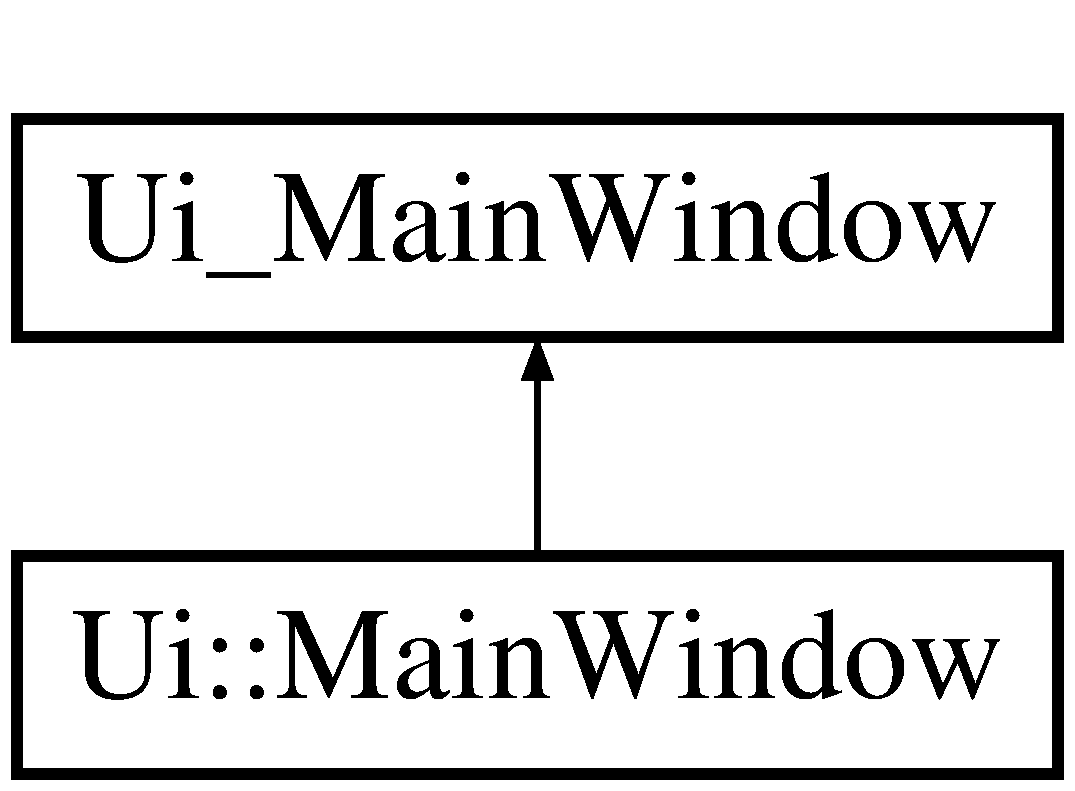
\includegraphics[height=2.000000cm]{class_ui_1_1_main_window}
\end{center}
\end{figure}
\subsection*{Additional Inherited Members}


The documentation for this class was generated from the following file\-:\begin{DoxyCompactItemize}
\item 
ui\-\_\-mainwindow.\-h\end{DoxyCompactItemize}

\hypertarget{class_main_window}{\section{Main\-Window Class Reference}
\label{class_main_window}\index{Main\-Window@{Main\-Window}}
}
Inheritance diagram for Main\-Window\-:\begin{figure}[H]
\begin{center}
\leavevmode
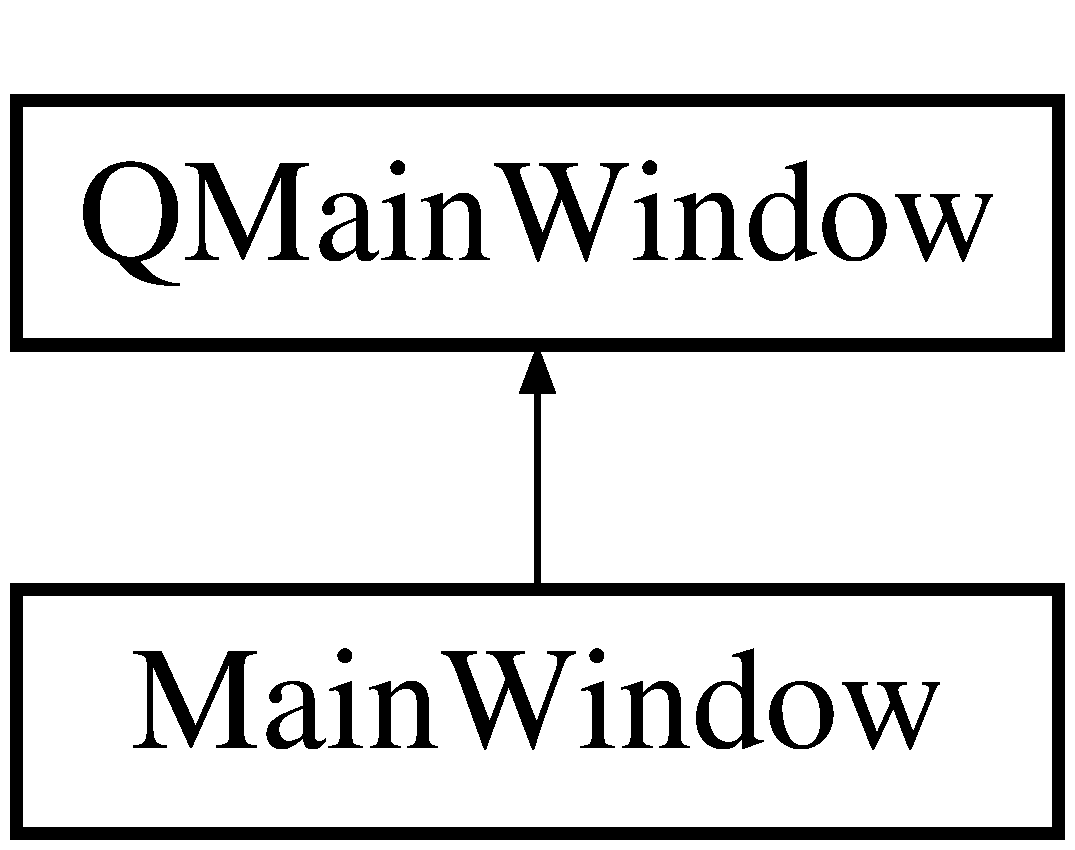
\includegraphics[height=2.000000cm]{class_main_window}
\end{center}
\end{figure}
\subsection*{Public Member Functions}
\begin{DoxyCompactItemize}
\item 
\hypertarget{class_main_window_a8b244be8b7b7db1b08de2a2acb9409db}{{\bfseries Main\-Window} (Q\-Widget $\ast$parent=0)}\label{class_main_window_a8b244be8b7b7db1b08de2a2acb9409db}

\end{DoxyCompactItemize}
\subsection*{Protected Member Functions}
\begin{DoxyCompactItemize}
\item 
\hypertarget{class_main_window_af4ca5d0d3d18ddcb7d54b6596bbf4797}{void {\bfseries change\-Event} (Q\-Event $\ast$e)}\label{class_main_window_af4ca5d0d3d18ddcb7d54b6596bbf4797}

\end{DoxyCompactItemize}


The documentation for this class was generated from the following files\-:\begin{DoxyCompactItemize}
\item 
mainwindow.\-h\item 
mainwindow.\-cpp\end{DoxyCompactItemize}

\hypertarget{class_mboj}{\section{Mboj Class Reference}
\label{class_mboj}\index{Mboj@{Mboj}}
}


trieda ktora sa stara o mechaniku boja  




{\ttfamily \#include $<$mboj.\-h$>$}

Inheritance diagram for Mboj\-:\begin{figure}[H]
\begin{center}
\leavevmode
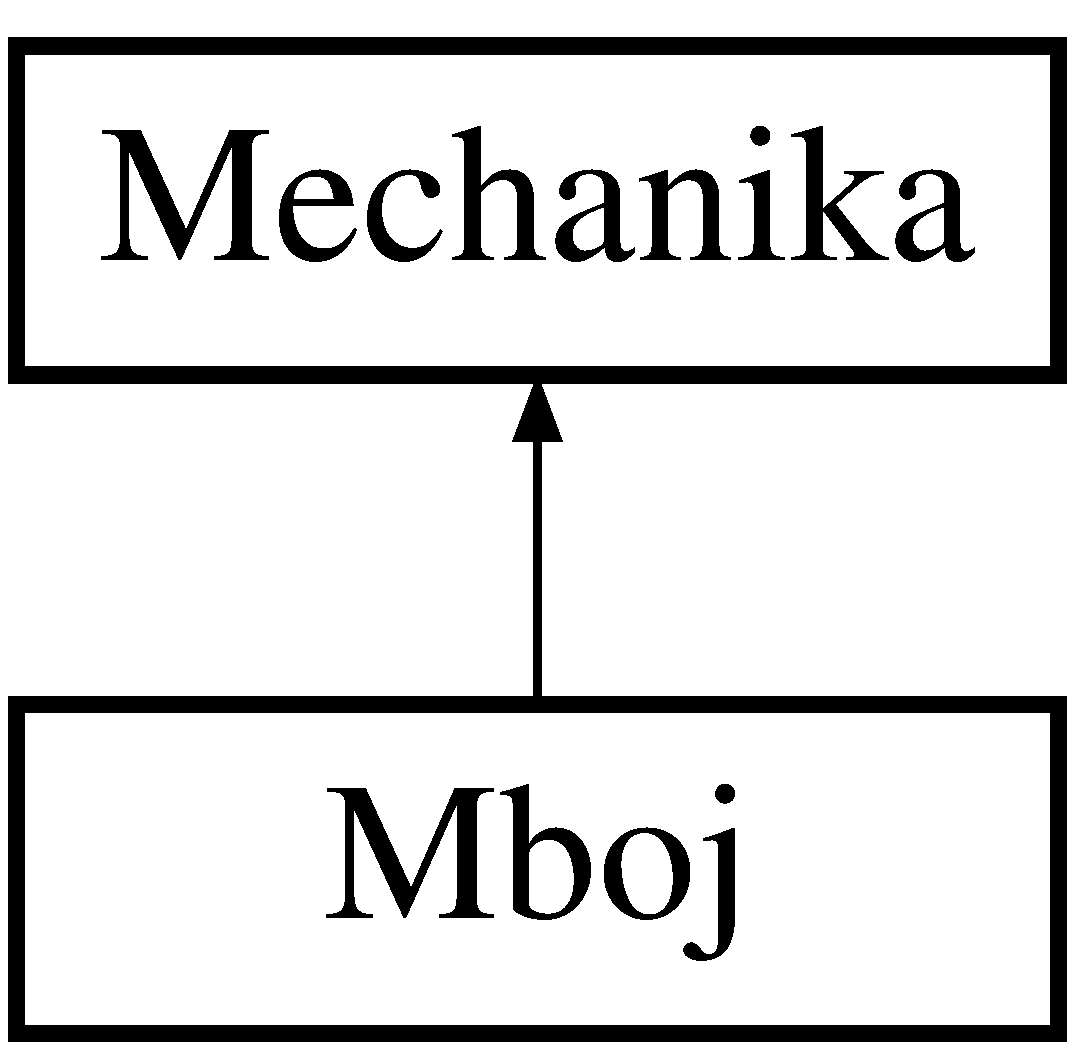
\includegraphics[height=2.000000cm]{class_mboj}
\end{center}
\end{figure}
\subsection*{Public Member Functions}
\begin{DoxyCompactItemize}
\item 
\hypertarget{class_mboj_a5c13a2d312899fbbc1a843bbdf2adae4}{\hyperlink{class_mboj_a5c13a2d312899fbbc1a843bbdf2adae4}{Mboj} (\hyperlink{class_lokacia}{Lokacia} $\ast$lok, \hyperlink{class_hrac}{Hrac} $\ast$hrac)}\label{class_mboj_a5c13a2d312899fbbc1a843bbdf2adae4}

\begin{DoxyCompactList}\small\item\em premenna obsahujuca uakzatel na lokaciu ktora sa prave pouziva \end{DoxyCompactList}\item 
\hypertarget{class_mboj_a443d2c40b47d934566b43f92f171ef08}{int \hyperlink{class_mboj_a443d2c40b47d934566b43f92f171ef08}{klavesa} (char key)}\label{class_mboj_a443d2c40b47d934566b43f92f171ef08}

\begin{DoxyCompactList}\small\item\em parametricky konstruktor \end{DoxyCompactList}\item 
\hypertarget{class_mboj_a94ea1bd996a151398df2892654263f93}{bool \hyperlink{class_mboj_a94ea1bd996a151398df2892654263f93}{suboj} ()}\label{class_mboj_a94ea1bd996a151398df2892654263f93}

\begin{DoxyCompactList}\small\item\em metoda ktora sa vola z Enginu pre spracovanie stlacenej klavesy \end{DoxyCompactList}\end{DoxyCompactItemize}


\subsection{Detailed Description}
trieda ktora sa stara o mechaniku boja 

The documentation for this class was generated from the following files\-:\begin{DoxyCompactItemize}
\item 
mboj.\-h\item 
mboj.\-cpp\end{DoxyCompactItemize}

\hypertarget{class_mechanika}{\section{Mechanika Class Reference}
\label{class_mechanika}\index{Mechanika@{Mechanika}}
}


treida ktora sa stara o celu mechaniku hry  




{\ttfamily \#include $<$Mechanika.\-h$>$}

Inheritance diagram for Mechanika\-:\begin{figure}[H]
\begin{center}
\leavevmode
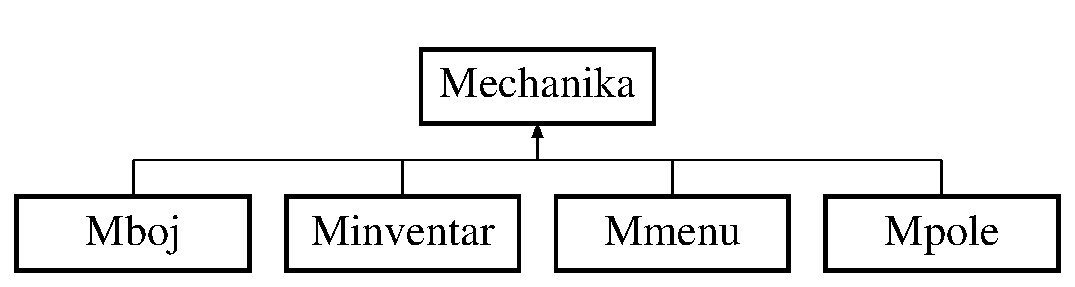
\includegraphics[height=2.000000cm]{class_mechanika}
\end{center}
\end{figure}
\subsection*{Public Member Functions}
\begin{DoxyCompactItemize}
\item 
\hypertarget{class_mechanika_ad7f0907c64f39a282c70d5349f0c7759}{\hyperlink{class_mechanika_ad7f0907c64f39a282c70d5349f0c7759}{Mechanika} ()}\label{class_mechanika_ad7f0907c64f39a282c70d5349f0c7759}

\begin{DoxyCompactList}\small\item\em premenna obsahujuca ukazatel an kreslic \end{DoxyCompactList}\item 
\hypertarget{class_mechanika_ac3f528e801774934865a993b4c9e3409}{virtual int {\bfseries klavesa} (char key)=0}\label{class_mechanika_ac3f528e801774934865a993b4c9e3409}

\end{DoxyCompactItemize}


\subsection{Detailed Description}
treida ktora sa stara o celu mechaniku hry 

The documentation for this class was generated from the following files\-:\begin{DoxyCompactItemize}
\item 
Mechanika.\-h\item 
Mechanika.\-cpp\end{DoxyCompactItemize}

\hypertarget{class_minventar}{\section{Minventar Class Reference}
\label{class_minventar}\index{Minventar@{Minventar}}
}


trieda ktora sa stara o pracu s inventarom  




{\ttfamily \#include $<$Minventar.\-h$>$}

Inheritance diagram for Minventar\-:\begin{figure}[H]
\begin{center}
\leavevmode
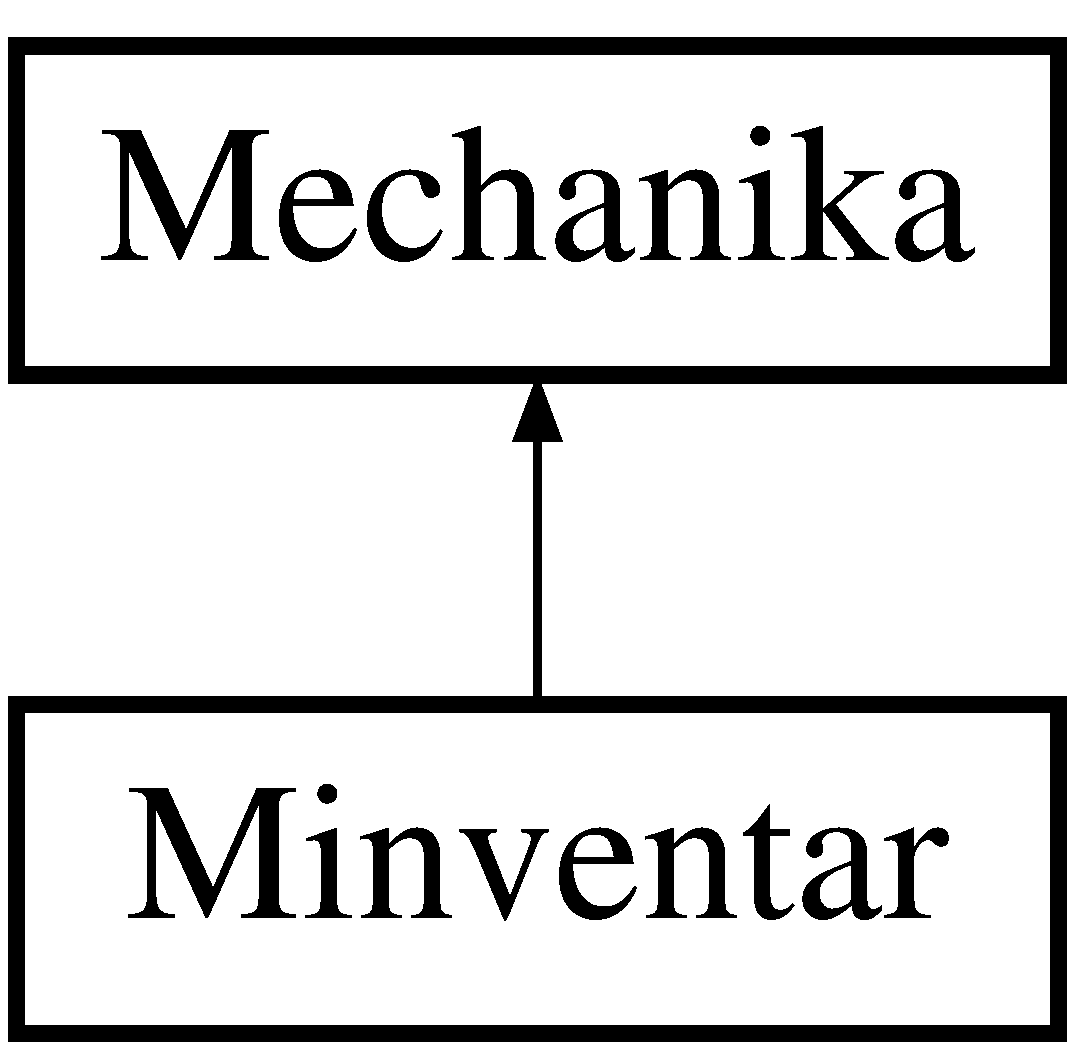
\includegraphics[height=2.000000cm]{class_minventar}
\end{center}
\end{figure}
\subsection*{Public Member Functions}
\begin{DoxyCompactItemize}
\item 
\hypertarget{class_minventar_a76050e1156ad9f99df1bc623322ef3fd}{int \hyperlink{class_minventar_a76050e1156ad9f99df1bc623322ef3fd}{klavesa} (char key)}\label{class_minventar_a76050e1156ad9f99df1bc623322ef3fd}

\begin{DoxyCompactList}\small\item\em konstruktor \end{DoxyCompactList}\end{DoxyCompactItemize}


\subsection{Detailed Description}
trieda ktora sa stara o pracu s inventarom 

The documentation for this class was generated from the following files\-:\begin{DoxyCompactItemize}
\item 
Minventar.\-h\item 
Minventar.\-cpp\end{DoxyCompactItemize}

\hypertarget{class_mmenu}{\section{Mmenu Class Reference}
\label{class_mmenu}\index{Mmenu@{Mmenu}}
}


trieda ktora sa stara o mechaniku hlavneho menu  




{\ttfamily \#include $<$Mmenu.\-h$>$}

Inheritance diagram for Mmenu\-:\begin{figure}[H]
\begin{center}
\leavevmode
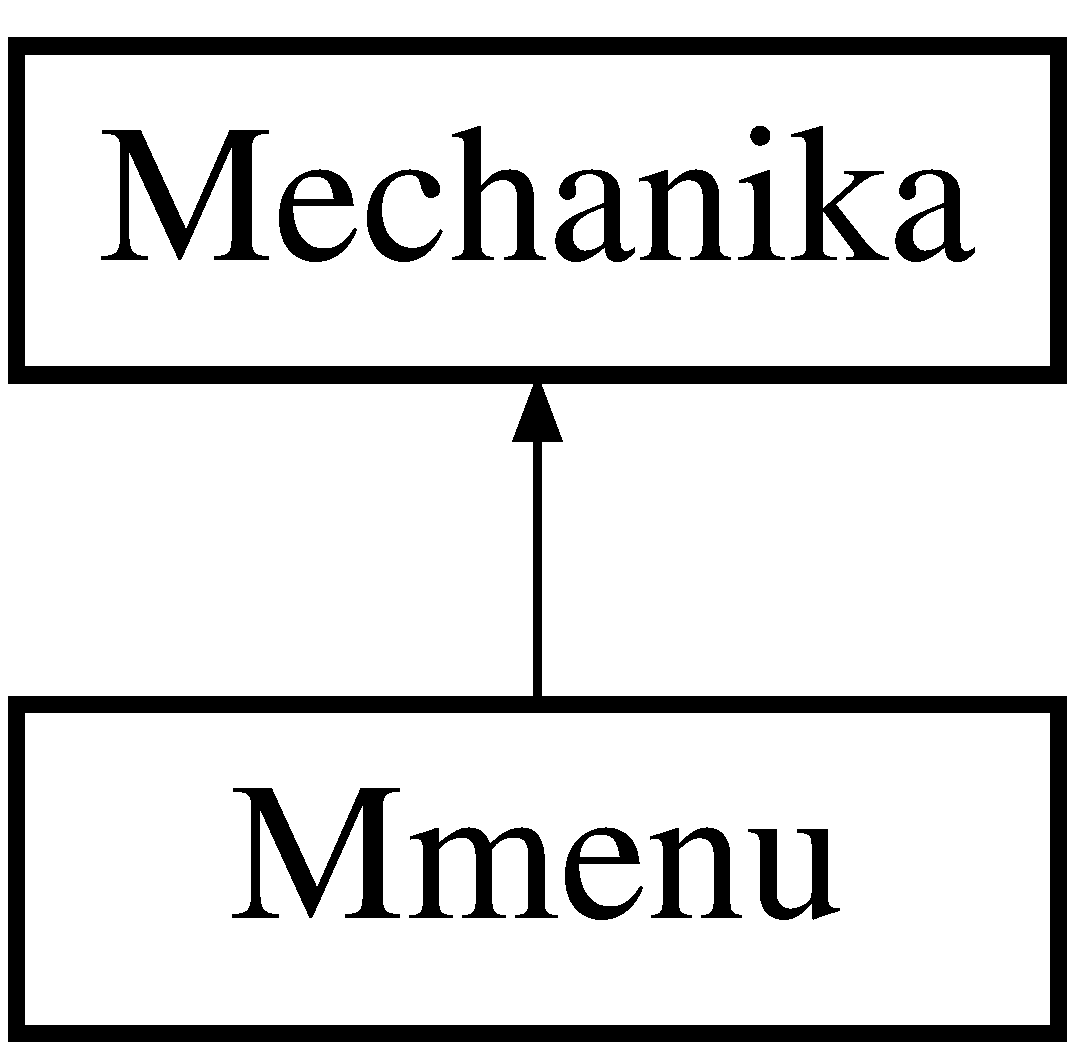
\includegraphics[height=2.000000cm]{class_mmenu}
\end{center}
\end{figure}
\subsection*{Public Member Functions}
\begin{DoxyCompactItemize}
\item 
\hypertarget{class_mmenu_adb3a3e05fbd1d06e92ac95fd5333110f}{int \hyperlink{class_mmenu_adb3a3e05fbd1d06e92ac95fd5333110f}{klavesa} (char key)}\label{class_mmenu_adb3a3e05fbd1d06e92ac95fd5333110f}

\begin{DoxyCompactList}\small\item\em konstruktor \end{DoxyCompactList}\item 
\hypertarget{class_mmenu_a9f03620caacd4206c698968f42925418}{void \hyperlink{class_mmenu_a9f03620caacd4206c698968f42925418}{dole} ()}\label{class_mmenu_a9f03620caacd4206c698968f42925418}

\begin{DoxyCompactList}\small\item\em metoda ktora sa stara o spracovanie klavesy ktora sa stlacila \end{DoxyCompactList}\item 
\hypertarget{class_mmenu_a469946d043186402bf546d74abdb7a1e}{void \hyperlink{class_mmenu_a469946d043186402bf546d74abdb7a1e}{hore} ()}\label{class_mmenu_a469946d043186402bf546d74abdb7a1e}

\begin{DoxyCompactList}\small\item\em metoda ktora sa stara o posun hore \end{DoxyCompactList}\item 
\hypertarget{class_mmenu_a2bbeb60a5baa8e9a1070db5695d2991b}{void \hyperlink{class_mmenu_a2bbeb60a5baa8e9a1070db5695d2991b}{potvrd} ()}\label{class_mmenu_a2bbeb60a5baa8e9a1070db5695d2991b}

\begin{DoxyCompactList}\small\item\em metoda ktora sa stara o posun dole \end{DoxyCompactList}\end{DoxyCompactItemize}


\subsection{Detailed Description}
trieda ktora sa stara o mechaniku hlavneho menu 

The documentation for this class was generated from the following files\-:\begin{DoxyCompactItemize}
\item 
Mmenu.\-h\item 
Mmenu.\-cpp\end{DoxyCompactItemize}

\hypertarget{class_mpole}{\section{Mpole Class Reference}
\label{class_mpole}\index{Mpole@{Mpole}}
}


trieda ktora sa stara o mechaniku herenho pola  




{\ttfamily \#include $<$Mpole.\-h$>$}

Inheritance diagram for Mpole\-:\begin{figure}[H]
\begin{center}
\leavevmode
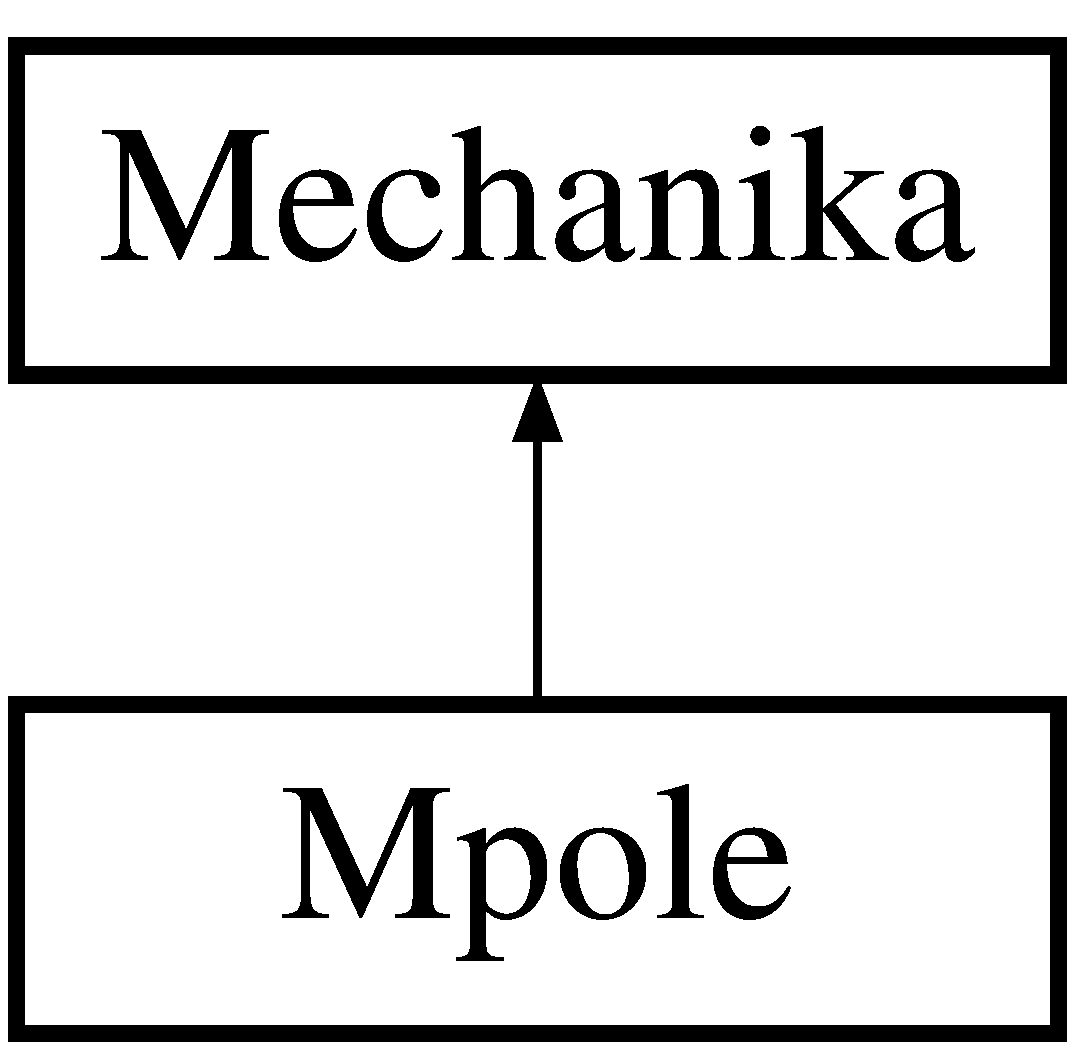
\includegraphics[height=2.000000cm]{class_mpole}
\end{center}
\end{figure}
\subsection*{Public Member Functions}
\begin{DoxyCompactItemize}
\item 
\hypertarget{class_mpole_afde0f9f2637657bc205f61564af2fa82}{\hyperlink{class_mpole_afde0f9f2637657bc205f61564af2fa82}{Mpole} (\hyperlink{class_lokacia}{Lokacia} $\ast$lok, \hyperlink{class_hrac}{Hrac} $\ast$hrac, int clokacia)}\label{class_mpole_afde0f9f2637657bc205f61564af2fa82}

\begin{DoxyCompactList}\small\item\em metoda ktora spracuva posun rhaca vlavo \end{DoxyCompactList}\item 
\hypertarget{class_mpole_aa133baee6547e3dfb4cf96d50ede2745}{int \hyperlink{class_mpole_aa133baee6547e3dfb4cf96d50ede2745}{klavesa} (char key)}\label{class_mpole_aa133baee6547e3dfb4cf96d50ede2745}

\begin{DoxyCompactList}\small\item\em pamatetricky konstruktor \end{DoxyCompactList}\item 
\hypertarget{class_mpole_a888a25f15e8bd4f5346b62d3cb64c33d}{bool \hyperlink{class_mpole_a888a25f15e8bd4f5346b62d3cb64c33d}{boj} ()}\label{class_mpole_a888a25f15e8bd4f5346b62d3cb64c33d}

\begin{DoxyCompactList}\small\item\em metoda ktora spracuva \end{DoxyCompactList}\item 
\hypertarget{class_mpole_ac63e2cb85985a843981dd05ab6e1e25a}{void \hyperlink{class_mpole_ac63e2cb85985a843981dd05ab6e1e25a}{objav} ()}\label{class_mpole_ac63e2cb85985a843981dd05ab6e1e25a}

\begin{DoxyCompactList}\small\item\em metoda ktora hlada vokoli hraca nepraitela \end{DoxyCompactList}\item 
\hypertarget{class_mpole_a4b8ec3339f346e769e8542b696cc8700}{void \hyperlink{class_mpole_a4b8ec3339f346e769e8542b696cc8700}{zdvihni} ()}\label{class_mpole_a4b8ec3339f346e769e8542b696cc8700}

\begin{DoxyCompactList}\small\item\em metoda ktora odkryva okolie od tmy \end{DoxyCompactList}\item 
\hypertarget{class_mpole_a4682f046dacdf4c3bdf3596113713fd3}{bool \hyperlink{class_mpole_a4682f046dacdf4c3bdf3596113713fd3}{postup} ()}\label{class_mpole_a4682f046dacdf4c3bdf3596113713fd3}

\begin{DoxyCompactList}\small\item\em metoda ktora vezme predmet z lokacie \end{DoxyCompactList}\end{DoxyCompactItemize}


\subsection{Detailed Description}
trieda ktora sa stara o mechaniku herenho pola 

The documentation for this class was generated from the following files\-:\begin{DoxyCompactItemize}
\item 
Mpole.\-h\item 
Mpole.\-cpp\end{DoxyCompactItemize}

\hypertarget{class_nepriatel}{\section{Nepriatel Class Reference}
\label{class_nepriatel}\index{Nepriatel@{Nepriatel}}
}


trieda ktora definu nepriatela  




{\ttfamily \#include $<$Nepriatel.\-h$>$}

\subsection*{Public Member Functions}
\begin{DoxyCompactItemize}
\item 
\hypertarget{class_nepriatel_ade9716acedbc03f644c5c780ead11de3}{\hyperlink{class_nepriatel_ade9716acedbc03f644c5c780ead11de3}{Nepriatel} (std\-::string meno, int utok, int obrana)}\label{class_nepriatel_ade9716acedbc03f644c5c780ead11de3}

\begin{DoxyCompactList}\small\item\em velkost zivota nepriatela \end{DoxyCompactList}\item 
\hypertarget{class_nepriatel_acc5fcfeffc566856e92a4388b6991c48}{int \hyperlink{class_nepriatel_acc5fcfeffc566856e92a4388b6991c48}{get\-Utok} ()}\label{class_nepriatel_acc5fcfeffc566856e92a4388b6991c48}

\begin{DoxyCompactList}\small\item\em parametrcky konstruktor \end{DoxyCompactList}\item 
\hypertarget{class_nepriatel_a6d2a11c1bc42f268b0ed053039825438}{int \hyperlink{class_nepriatel_a6d2a11c1bc42f268b0ed053039825438}{get\-Obrana} ()}\label{class_nepriatel_a6d2a11c1bc42f268b0ed053039825438}

\begin{DoxyCompactList}\small\item\em metoda ktora vrati utok nepraitela \end{DoxyCompactList}\item 
\hypertarget{class_nepriatel_a2420d033a88248842ea9f272eeb3ee1b}{int \hyperlink{class_nepriatel_a2420d033a88248842ea9f272eeb3ee1b}{get\-Zivot} ()}\label{class_nepriatel_a2420d033a88248842ea9f272eeb3ee1b}

\begin{DoxyCompactList}\small\item\em metoda ktora vracia obranu \end{DoxyCompactList}\item 
\hypertarget{class_nepriatel_ab33a949533fafe3c33c7e17a17fa4831}{std\-::string \hyperlink{class_nepriatel_ab33a949533fafe3c33c7e17a17fa4831}{get\-Meno} ()}\label{class_nepriatel_ab33a949533fafe3c33c7e17a17fa4831}

\begin{DoxyCompactList}\small\item\em metoda ktora varcia zivot \end{DoxyCompactList}\item 
\hypertarget{class_nepriatel_a750713aaba696e6fba26ae688b6a9ecb}{void \hyperlink{class_nepriatel_a750713aaba696e6fba26ae688b6a9ecb}{set\-Zivot} (int zivot)}\label{class_nepriatel_a750713aaba696e6fba26ae688b6a9ecb}

\begin{DoxyCompactList}\small\item\em metoda ktora vracia meno nepriatela \end{DoxyCompactList}\item 
\hypertarget{class_nepriatel_a1228bd712885a63bbb05d6c9e39108fc}{\hyperlink{class_nepriatel_a1228bd712885a63bbb05d6c9e39108fc}{Nepriatel} (const \hyperlink{class_nepriatel}{Nepriatel} \&vzor)}\label{class_nepriatel_a1228bd712885a63bbb05d6c9e39108fc}

\begin{DoxyCompactList}\small\item\em metoda ktora upravuje zivot \end{DoxyCompactList}\end{DoxyCompactItemize}


\subsection{Detailed Description}
trieda ktora definu nepriatela 

The documentation for this class was generated from the following files\-:\begin{DoxyCompactItemize}
\item 
Nepriatel.\-h\item 
Nepriatel.\-cpp\end{DoxyCompactItemize}

\hypertarget{struct_pozicia}{\section{Pozicia Struct Reference}
\label{struct_pozicia}\index{Pozicia@{Pozicia}}
}


struct definujuci poziciu  




{\ttfamily \#include $<$Pozicia.\-h$>$}

\subsection*{Public Member Functions}
\begin{DoxyCompactItemize}
\item 
\hypertarget{struct_pozicia_a9504f32b736dd8851a4d2dc6f879f747}{{\bfseries Pozicia} (const int x, const int y)}\label{struct_pozicia_a9504f32b736dd8851a4d2dc6f879f747}

\end{DoxyCompactItemize}
\subsection*{Public Attributes}
\begin{DoxyCompactItemize}
\item 
\hypertarget{struct_pozicia_a6e6399f4cb1223dc64b79c3193576de2}{int {\bfseries x}}\label{struct_pozicia_a6e6399f4cb1223dc64b79c3193576de2}

\item 
\hypertarget{struct_pozicia_a9a149a110efda12e363480be0492545d}{int {\bfseries y}}\label{struct_pozicia_a9a149a110efda12e363480be0492545d}

\end{DoxyCompactItemize}


\subsection{Detailed Description}
struct definujuci poziciu 

The documentation for this struct was generated from the following file\-:\begin{DoxyCompactItemize}
\item 
Pozicia.\-h\end{DoxyCompactItemize}

\hypertarget{class_predmet}{\section{Predmet Class Reference}
\label{class_predmet}\index{Predmet@{Predmet}}
}
Inheritance diagram for Predmet\-:\begin{figure}[H]
\begin{center}
\leavevmode
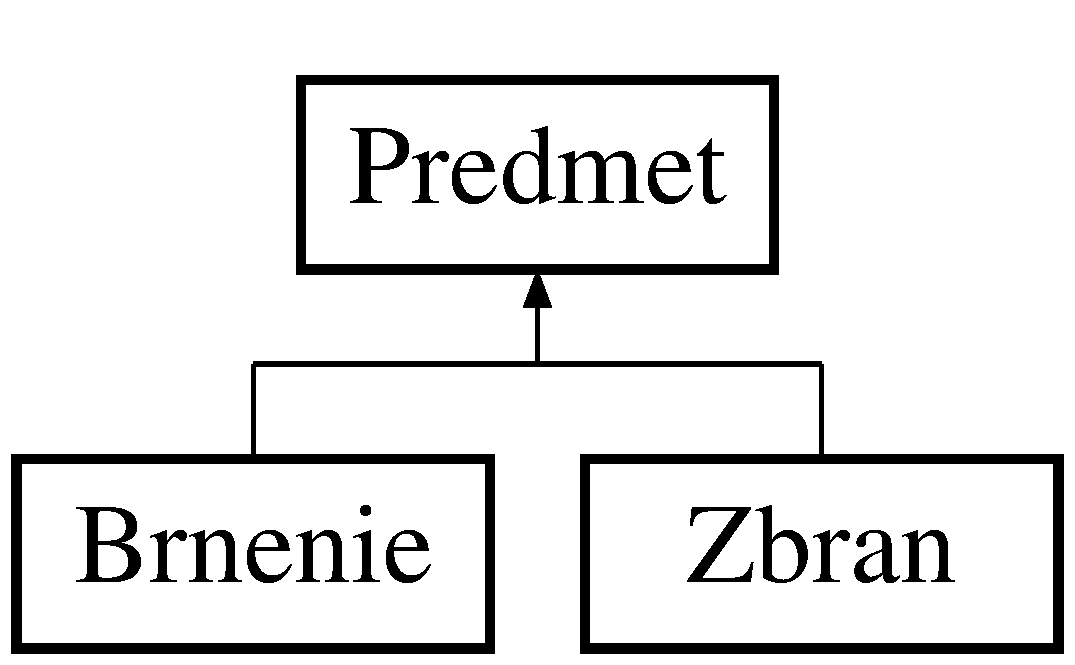
\includegraphics[height=2.000000cm]{class_predmet}
\end{center}
\end{figure}
\subsection*{Public Member Functions}
\begin{DoxyCompactItemize}
\item 
\hypertarget{class_predmet_ad4c245d0915fffcb7cd6e90073a2984b}{\hyperlink{class_predmet_ad4c245d0915fffcb7cd6e90073a2984b}{Predmet} ()}\label{class_predmet_ad4c245d0915fffcb7cd6e90073a2984b}

\begin{DoxyCompactList}\small\item\em sila predmetu (brnenie alebo zbran) \end{DoxyCompactList}\item 
\hypertarget{class_predmet_a416eba4ff016ba3bbeb32988e49492f7}{std\-::string \hyperlink{class_predmet_a416eba4ff016ba3bbeb32988e49492f7}{get\-Nazov} ()}\label{class_predmet_a416eba4ff016ba3bbeb32988e49492f7}

\begin{DoxyCompactList}\small\item\em konstruktor ktori sa nikdy nepouzije \end{DoxyCompactList}\item 
\hypertarget{class_predmet_a10937e2b58fbab9114ca6dbc03f2d4b7}{int \hyperlink{class_predmet_a10937e2b58fbab9114ca6dbc03f2d4b7}{get\-Sila} ()}\label{class_predmet_a10937e2b58fbab9114ca6dbc03f2d4b7}

\begin{DoxyCompactList}\small\item\em metoda vracia atribut m\-\_\-nazov \end{DoxyCompactList}\end{DoxyCompactItemize}
\subsection*{Protected Attributes}
\begin{DoxyCompactItemize}
\item 
\hypertarget{class_predmet_aad5beccc8ba4a990a8f129f281dbc158}{std\-::string {\bfseries m\-\_\-nazov}}\label{class_predmet_aad5beccc8ba4a990a8f129f281dbc158}

\item 
\hypertarget{class_predmet_af9c5542008e72261515a10ade519e241}{int \hyperlink{class_predmet_af9c5542008e72261515a10ade519e241}{m\-\_\-sila}}\label{class_predmet_af9c5542008e72261515a10ade519e241}

\begin{DoxyCompactList}\small\item\em nazov predmetu (brnenia alebo zbrane) \end{DoxyCompactList}\end{DoxyCompactItemize}


The documentation for this class was generated from the following files\-:\begin{DoxyCompactItemize}
\item 
Predmet.\-h\item 
Predmet.\-cpp\end{DoxyCompactItemize}

\hypertarget{class_ui___main_window}{\section{Ui\-\_\-\-Main\-Window Class Reference}
\label{class_ui___main_window}\index{Ui\-\_\-\-Main\-Window@{Ui\-\_\-\-Main\-Window}}
}
Inheritance diagram for Ui\-\_\-\-Main\-Window\-:\begin{figure}[H]
\begin{center}
\leavevmode
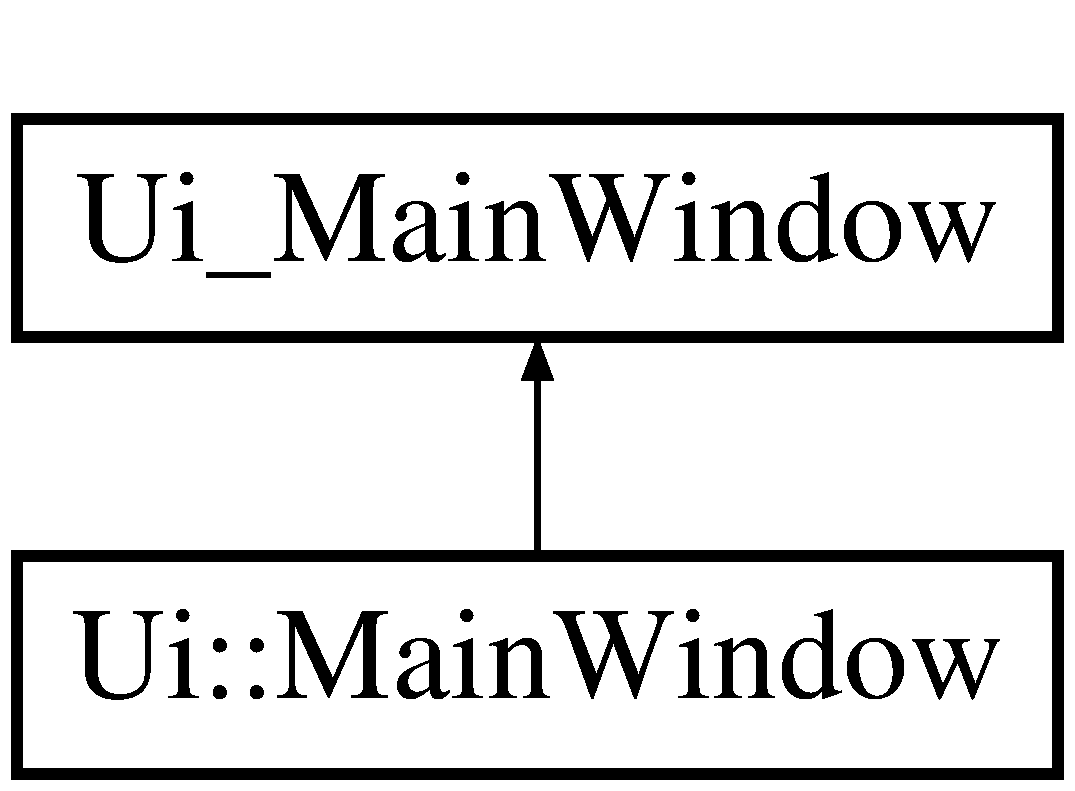
\includegraphics[height=2.000000cm]{class_ui___main_window}
\end{center}
\end{figure}
\subsection*{Public Member Functions}
\begin{DoxyCompactItemize}
\item 
\hypertarget{class_ui___main_window_acf4a0872c4c77d8f43a2ec66ed849b58}{void {\bfseries setup\-Ui} (Q\-Main\-Window $\ast$\hyperlink{class_main_window}{Main\-Window})}\label{class_ui___main_window_acf4a0872c4c77d8f43a2ec66ed849b58}

\item 
\hypertarget{class_ui___main_window_a097dd160c3534a204904cb374412c618}{void {\bfseries retranslate\-Ui} (Q\-Main\-Window $\ast$\hyperlink{class_main_window}{Main\-Window})}\label{class_ui___main_window_a097dd160c3534a204904cb374412c618}

\end{DoxyCompactItemize}
\subsection*{Public Attributes}
\begin{DoxyCompactItemize}
\item 
\hypertarget{class_ui___main_window_a2be1c24ec9adfca18e1dcc951931457f}{Q\-Menu\-Bar $\ast$ {\bfseries menu\-Bar}}\label{class_ui___main_window_a2be1c24ec9adfca18e1dcc951931457f}

\item 
\hypertarget{class_ui___main_window_a5172877001c8c7b4e0f6de50421867d1}{Q\-Tool\-Bar $\ast$ {\bfseries main\-Tool\-Bar}}\label{class_ui___main_window_a5172877001c8c7b4e0f6de50421867d1}

\item 
\hypertarget{class_ui___main_window_a30075506c2116c3ed4ff25e07ae75f81}{Q\-Widget $\ast$ {\bfseries central\-Widget}}\label{class_ui___main_window_a30075506c2116c3ed4ff25e07ae75f81}

\item 
\hypertarget{class_ui___main_window_a50fa481337604bcc8bf68de18ab16ecd}{Q\-Status\-Bar $\ast$ {\bfseries status\-Bar}}\label{class_ui___main_window_a50fa481337604bcc8bf68de18ab16ecd}

\end{DoxyCompactItemize}


The documentation for this class was generated from the following file\-:\begin{DoxyCompactItemize}
\item 
ui\-\_\-mainwindow.\-h\end{DoxyCompactItemize}

\hypertarget{class_zbran}{\section{Zbran Class Reference}
\label{class_zbran}\index{Zbran@{Zbran}}
}
Inheritance diagram for Zbran\-:\begin{figure}[H]
\begin{center}
\leavevmode
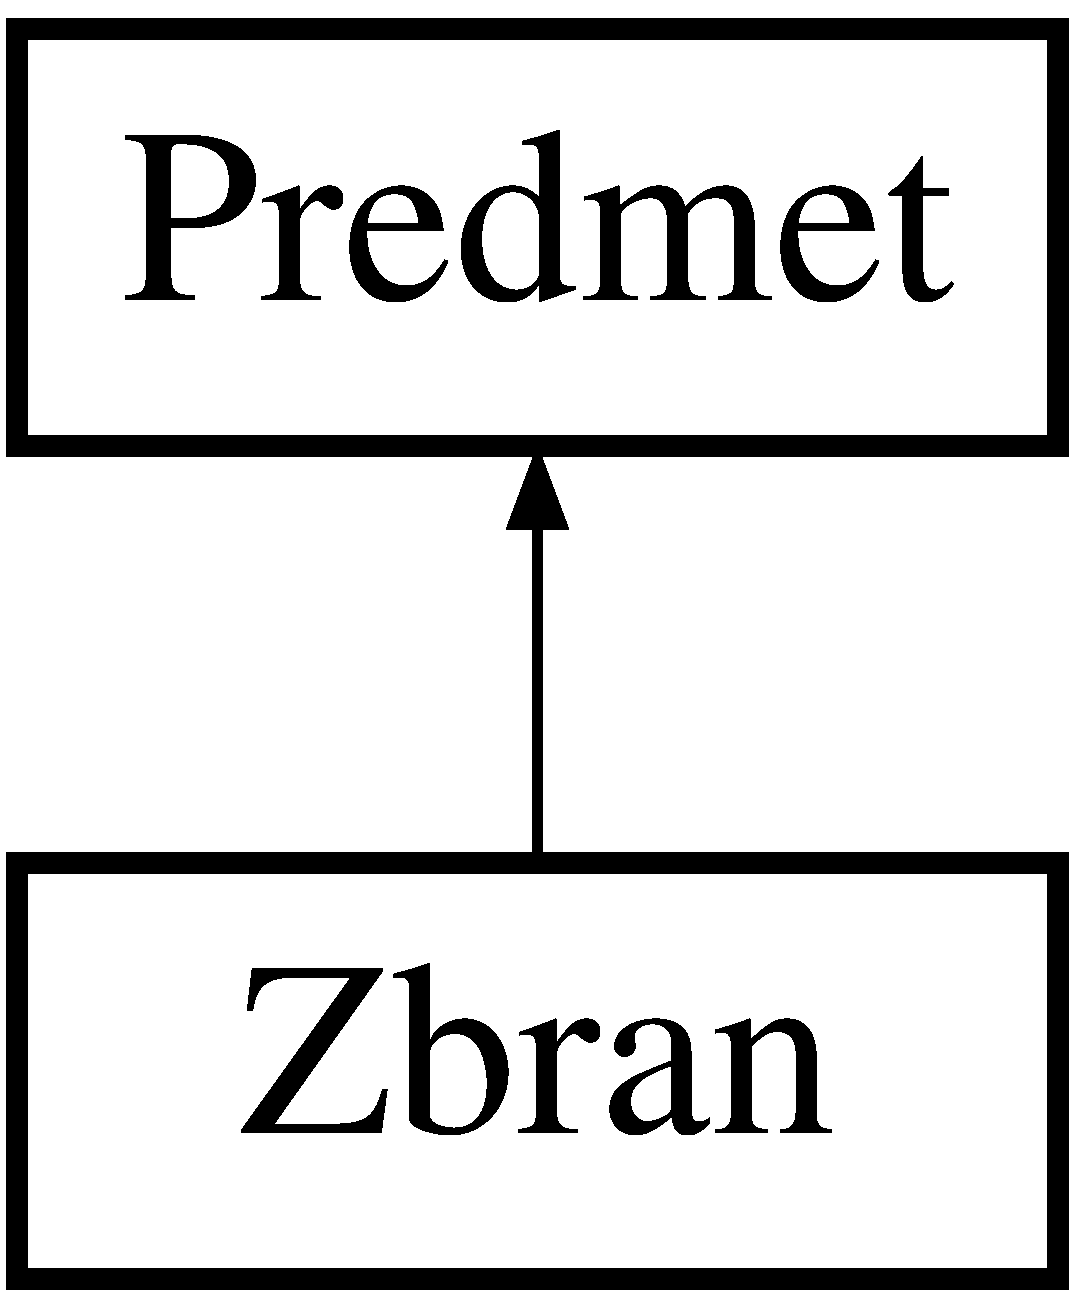
\includegraphics[height=2.000000cm]{class_zbran}
\end{center}
\end{figure}
\subsection*{Public Member Functions}
\begin{DoxyCompactItemize}
\item 
\hypertarget{class_zbran_a5f5db62ac980f4c15e3541d8a67de9b5}{{\bfseries Zbran} (std\-::string nazov, int sila)}\label{class_zbran_a5f5db62ac980f4c15e3541d8a67de9b5}

\end{DoxyCompactItemize}
\subsection*{Additional Inherited Members}


The documentation for this class was generated from the following files\-:\begin{DoxyCompactItemize}
\item 
Zbran.\-h\item 
Zbran.\-cpp\end{DoxyCompactItemize}

%--- End generated contents ---

% Index
\newpage
\phantomsection
\addcontentsline{toc}{chapter}{Index}
\printindex

\end{document}
